\documentclass[12pt]{article}

% ====================================================================
% PHAGE THERAPY FOR MDR/XDR/PDR PSEUDOMONAS AERUGINOSA
% Systematic Review and Meta-Analysis of Proportions
%
% Preamble adapted from .claude/rules/working-paper-format.md (the
% project's economics-default reference preamble) for a biomedical
% systematic review / meta-analysis. See the "Preamble Deviations"
% note at the bottom of this file for what was kept, dropped, or
% changed and why.
% ====================================================================

% ====== Page Layout and Basic Formatting ======
\usepackage[left=1.0in,right=1.0in,top=1.0in,bottom=1.0in]{geometry}
\usepackage{setspace}
\doublespacing
\usepackage{fancyhdr}
\pagestyle{fancy}
\fancyhf{}
\fancyfoot[C]{\thepage}
\renewcommand{\headrulewidth}{0pt}

% ====== Typography and Fonts ======
\usepackage{lmodern}
\usepackage[T1]{fontenc}
\usepackage{microtype}
% fontspec + the OpenType Latin Modern Roman font: XeLaTeX-native Unicode
% coverage for glyphs the legacy 8-bit T1/lmodern (ec-lmr) fonts lack, e.g.
% c-acute (\'{c}) in the Savovi{\'c} citation -- otherwise "Missing character"
\usepackage{fontspec}
\setmainfont{Latin Modern Roman}

% ====== Math Packages ======
\usepackage{amsmath, amssymb}

% ====== Color (base dependency for tabularray/hyperref internals) ======
\usepackage{xcolor}

% ====== Table Packages ======
\usepackage{array, booktabs}
\usepackage[flushleft]{threeparttable}
\usepackage{siunitx}
\usepackage{tabularray}
\UseTblrLibrary{booktabs, siunitx}

% ====== Figure and Caption Packages ======
\usepackage{graphicx, subcaption}
\usepackage{caption}
\captionsetup{font=small, labelfont=bf, justification=justified}
\captionsetup[figure]{labelfont=bf}
% tikz: used only for the hand-built PRISMA 2020 flow diagram (Figure 1),
% which is not R-generated data output, so it doesn't go through the
% R figure pipeline like the forest/funnel plots
\usepackage{tikz}
\usetikzlibrary{arrows.meta, positioning, fit}

% ====== List Formatting ======
\usepackage{enumitem}

% ====== Bibliography (biblatex + biber) ======
\usepackage{xurl}
\usepackage[backend=biber,
            style=authoryear,
            maxcitenames=3,
            mincitenames=1,
            maxbibnames=99,
            giveninits=true,
            uniquename=false,
            uniquelist=true,
            dashed=false,
            urldate=long,
            url=true,
            natbib=true]{biblatex}
\addbibresource{Bibliography_base.bib}
% Bibliography_base.bib's `note` field holds this project's internal extraction/
% verification audit trail (source, date, PMID, reviewer rationale) -- useful for
% this review's own provenance tracking, not reader-facing bibliographic content.
% biblatex's authoryear style prints `note` by default; suppress it here rather
% than deleting the field, so the audit trail stays intact in the .bib source.
\AtEveryBibitem{\clearfield{note}}

% URL bleeding fixes
\setcounter{biburllcpenalty}{7000}
\setcounter{biburlucpenalty}{8000}
\setcounter{biburlnumpenalty}{9000}

% ====== Hyperref (loaded second-to-last) ======
\usepackage[hidelinks, breaklinks, colorlinks=false]{hyperref}

% ====== Cleveref (loaded immediately after hyperref) ======
\usepackage[nameinlink]{cleveref}

\title{Phage Therapy for MDR/XDR/PDR \textit{Pseudomonas aeruginosa}: A Systematic Review and Meta-Analysis of Proportions}

\author{%
[Author Name(s)]\thanks{Universidad Cat\'olica de Cuenca, Cuenca, Ecuador. Corresponding author: [email address TBD]. Full author list, affiliations, and contribution statement (per ICMJE criteria) to be finalized before journal submission --- no specific authorship has been established as of this draft.}%
}

\date{\today}

\begin{document}

\maketitle
\thispagestyle{empty}

\begin{abstract}
\noindent \singlespacing
Background: Multidrug-resistant (MDR), extensively drug-resistant (XDR), and pandrug-resistant (PDR) \textit{Pseudomonas aeruginosa} is a WHO priority pathogen with few options. Phage therapy has expanded from compassionate use to early-phase trials without resistance- or route-stratified synthesis. Methods: We conducted a PRISMA 2020 meta-analysis of proportions (binomial-normal GLMM), pooling clinical success, safety, eradication, and mortality across phage-therapy studies of MDR/XDR/PDR \textit{P.\ aeruginosa}, stratified by resistance category, route, and modality. Results: Twenty-nine pooling-eligible study-arms (25 studies, 107 patients) yielded clinical success in 77.3\% (95\% CI 65.4--86.4\%). Of 37 pre-specified strata, 15 met threshold, including a single-cohort MDR estimate poolable only under author-reported labels: MDR clinical success 75.7\% (95\% CI 57.8--87.6\%). XDR, PDR, most routes, and monotherapy remained below threshold. Peters' test (appropriate for proportions) showed no significant small-study asymmetry for any tested outcome (all p>0.2). Conclusions: The MDR estimate is achievable but fragile; the MDR-versus-XDR comparison remains open.
\end{abstract}

\vspace{1em}
\noindent \textbf{Keywords:} Bacteriophages; Pseudomonas aeruginosa; Drug Resistance, Multiple, Bacterial; Phage Therapy; Systematic Reviews as Topic; Meta-Analysis as Topic

\newpage
\setcounter{page}{1}

\section{Introduction}
\label{sec:introduction}

\textit{Pseudomonas aeruginosa} appears on the World Health Organization's priority list of antibiotic-resistant pathogens because of its capacity to accumulate resistance to nearly every class of antipseudomonal agent \parencite{Tacconelli2018_who}. That framing needs one correction, and it cuts against rather than for the urgency of this review's question: the 2024 update to the priority list \emph{downgraded} carbapenem-resistant \textit{P.\ aeruginosa} from Critical to High \parencite{WHO2024_bppl}. We note it explicitly rather than quietly citing the superseded 2018 list. The organism remains a High-priority pathogen for which salvage options are genuinely scarce, which is sufficient motivation; overstating its rank is not necessary and would not survive review.

A second correction is owed to the premise itself. It is no longer accurate to say the antipseudomonal pipeline has stalled: ceftolozane--tazobactam, ceftazidime--avibactam, imipenem--relebactam and cefiderocol all reached clinical use in the last decade and between them recovered activity against many isolates that older definitions call multidrug-resistant. The scarcity this review addresses is therefore not an absence of new agents but the narrower and harder situation those agents leave behind --- the patient in whom they have also failed, or cannot be used. That distinction has a formal counterpart. The Magiorakos categories (MDR/XDR/PDR) count how many antimicrobial \emph{categories} an isolate resists, a measure the new agents have made less decision-relevant; \textcite{Kadri2018_dtr} instead define \emph{difficult-to-treat resistance} (DTR) as non-susceptibility to all \emph{first-line} agents --- the carbapenem, extended-spectrum cephalosporin, $\beta$-lactam/$\beta$-lactamase-inhibitor and fluoroquinolone categories --- which is the point at which a clinician is forced onto reserve therapy. The reserve agents themselves, which \citeauthor{Kadri2018_dtr} name as aminoglycosides, polymyxins and tigecycline, do \emph{not} enter the determination: an isolate susceptible only to colistin is DTR precisely because colistin is what is left. DTR, not MDR, is the category current guidance uses for treatment decisions in \textit{P.\ aeruginosa}. We retain the Magiorakos axis as primary because it is what the published literature reports, and we carry DTR as a separate stratum precisely to show what that reporting practice costs (Sections~\ref{sec:methods-eligibility} and~\ref{sec:results-synthesis}). Once an isolate meets criteria for multidrug resistance (MDR), extensive drug resistance (XDR), or pandrug resistance (PDR) under the Magiorakos framework \parencite{Magiorakos2012_mdrxdr}, treatment options narrow quickly. The antipseudomonal development pipeline has not kept pace, and bacteriophage therapy---administered alone or alongside antibiotics---has moved from isolated compassionate-use reports toward a small but growing set of early-phase trials as a salvage option for infections that no longer respond to conventional regimens.

This evidence base has already been synthesized many times. Since \textcite{ElHaddad2019_eskape} reviewed phage therapy against ESKAPE pathogens in 2019, at least eight further systematic reviews, meta-analyses, and scoping reviews of human phage therapy have appeared, including a large multi-author synthesis in \textit{Lancet Infectious Diseases} \parencite{Uyttebroek2022_lancetid} and, most recently, an individual-patient-data meta-analysis of 130 studies spanning multiple pathogens \parencite{Liu2025_ijaa}. None restricts its pooling to \textit{P. aeruginosa} specifically, and none stratifies pooled outcomes by resistance category or by route of phage administration---the two variables clinicians most need resolved when choosing a regimen for a given patient and infection site.

Our original aim was narrower still: to compare, within the same studies, phage-antibiotic combination therapy against antibiotic monotherapy for MDR/XDR/PDR \textit{P. aeruginosa} and to estimate a pooled effect size for clinical success. A systematic search of PubMed/MEDLINE and ClinicalTrials.gov found no study reporting both a genuine antibiotic-monotherapy arm and a phage-antibiotic combination arm in a \textit{P. aeruginosa}-specific, MDR/XDR/PDR-defined population, so this comparison could not be constructed under any available within-study design. We therefore reframed the review around pooled proportions rather than a paired effect estimate: the proportion of patients achieving clinical success and the proportion experiencing a safety event across the single-arm and comparative studies that do exist, with pre-specified stratification by resistance category (MDR, XDR, or PDR), route of administration, and treatment modality (antibiotic monotherapy vs.\ phage-antibiotic combination).

Specifically, among patients with MDR, XDR, or PDR \textit{P. aeruginosa} infections treated with bacteriophage therapy, we asked: what proportion achieve clinical success, what proportion experience an adverse event, and do these proportions differ by resistance category, administration route, or treatment modality?

We found the current evidence base able to answer only part of the stratified question it was designed to ask. Pooling across all included studies yielded a clinical-success proportion of \CsOverallEst(\CsOverallCI), directionally consistent with the high success rates reported by prior, non-stratified syntheses---but this figure comes from a compassionate-use population selected for refractory infection after antibiotic failure and should not be read as evidence that phage therapy outperforms, or underperforms, any comparator. Stratification succeeded, but only just, for one resistance class: MDR isolates specifically now have a pooled estimate (\CsResMDREstCI clinical success). We present this as a single-cohort characterization rather than a headline achievement: it draws two-thirds of its patients from one cohort and clears the pre-specified evidentiary threshold only under author-reported resistance labels---restricted to independently re-derived classifications, the MDR cell collapses from \ClassMDRStudiesAll studies and \ClassMDRPatientsAll patients to \ClassMDRStudiesVerified studies and \ClassMDRPatientsVerified patients, and cannot be pooled at all. XDR, PDR, every specific administration route, and modality all fell short of the number of studies and patients needed for a stable pooled estimate, and despite a targeted search, no eligible antibiotic-monotherapy arm was identified---so the MDR-versus-XDR comparison that motivated this review remains unanswered even though MDR alone is not. Documenting exactly which parts of this stratified question the current evidence can and cannot answer, rather than forcing an estimate the data cannot support or dismissing the one part that succeeded, is the contribution of this review.


\section{Methods}
\label{sec:methods}

This review follows the PRISMA 2020 reporting standard \parencite{Page2021_prisma} and the methodological guidance of the Cochrane Handbook \parencite{Higgins2023_cochranehandbook}, adapted throughout for a synthesis of proportions rather than a synthesis of comparative treatment effects, for the reasons given in the Introduction. Every design choice below---eligibility, search, extraction, risk-of-bias assessment, and the pooling model itself---was fixed before formal data extraction began, and is reported here exactly as specified, including the places where the evidence base did not cooperate with the plan and the places where this review's own execution fell short of its own plan.

\subsection{Protocol and Registration}
\label{sec:methods-protocol}

This review was not registered in PROSPERO before literature screening or data extraction began. The design pivoted once during discovery, from a comparative-effect meta-analysis (phage-antibiotic combination versus antibiotic monotherapy) to the stratified meta-analysis of proportions reported here, after two independent search rounds found zero to one qualifying dual-arm comparative studies for MDR/XDR \textit{P.\ aeruginosa}. That pivot needed to happen before a protocol could be written that the team would not have to immediately amend. That scoping work included four rounds of literature searching (Section~\ref{sec:methods-search}) and one informal, single-reviewer screening pass of a 201-document local PDF corpus, conducted against this review's PICO criteria but without the dual-independent review PROSPERO registration presumes. PROSPERO's own policy does not prohibit preliminary scoping before registration; it prohibits registering a protocol once data extraction and synthesis are already substantively underway. By that standard, registration remained available through the design-pivot and literature-search stages of this project, and did not occur. Data extraction and the statistical synthesis reported in Results proceeded before a protocol was ever submitted -- a genuine deviation from prospective registration -- and that extraction itself was conducted by a single reviewer rather than the dual-independent process a registered protocol would specify (Sections~\ref{sec:methods-selection} and \ref{sec:methods-extraction}). The full scoping timeline is as follows: two PubMed/ClinicalTrials.gov search rounds and a targeted third and fourth round (Section~\ref{sec:methods-search}), one ad hoc single-reviewer PDF screen, and the resulting design pivot, all preceded any protocol filing, and no protocol was filed before extraction and pooling were carried out. We recommend retrospective PROSPERO registration disclosing this exact sequence before this review is submitted for publication.

\subsection{Eligibility Criteria}
\label{sec:methods-eligibility}

Eligibility follows a PICO framework, broadened partway through discovery once the design pivoted from a comparative-effect estimand to a proportion estimand (Section~\ref{sec:methods-protocol}): under the original comparative-only design, a study needed both a phage-containing arm and a within-study antibiotic-monotherapy arm to qualify, a requirement that essentially no study in this literature satisfies. Under the current design, single-arm and comparative studies are equally eligible, because every outcome is computed at the study-arm level rather than as a paired comparison.

\begin{itemize}
\item \textbf{Population.} Patients with an infection attributed to multidrug-resistant (MDR), extensively drug-resistant (XDR), or pandrug-resistant (PDR) \textit{Pseudomonas aeruginosa}, classified per the \textcite{Magiorakos2012_mdrxdr} criteria where the primary study reports sufficient susceptibility data, and per the study's own MDR/XDR/PDR label otherwise (Section~\ref{sec:methods-extraction}). Two boundary cases must be distinguished, and this review treats them differently. Where a study reports susceptibility data that \emph{positively fail} the Magiorakos threshold, the arm does not meet the population criterion and is excluded, whatever the study's own descriptive language; one arm is excluded on exactly this ground (Section~\ref{sec:results-selection}). Where a study reports \emph{no} resistance information, the arm is retained and coded \emph{not classifiable} rather than excluded, because absence of a reported susceptibility panel is not evidence of susceptibility, and excluding on missing data would discard entire trials for a reporting omission. We state plainly that this second rule makes the analysed population broader than the criterion as written: the not-classifiable arms are predominantly trial populations enrolled on the basis of \textit{P.\ aeruginosa} infection or chronic colonization without any resistance requirement, so pooled ``overall'' estimates should be read as describing phage therapy in \textit{P.\ aeruginosa} infection generally, not exclusively in the resistant population named in this review's title. Resistance-stratified estimates carry no such ambiguity. A sensitivity analysis quantifies the consequence (Section~\ref{sec:results-robustness}).
\item \textbf{Intervention.} Bacteriophage therapy, administered as monotherapy or adjunctively with antibiotics, by any route.
\item \textbf{Comparator.} None required. Where a genuine within-study comparator exists (an antibiotic-only or placebo arm), it is retained and reported, but its presence is not an eligibility condition.
\item \textbf{Outcomes.} Clinical success and any adverse event (primary); microbiological eradication, mortality, length of hospitalization, and resistance emergence during treatment (secondary), each defined per the primary study's own reporting given the expected heterogeneity in how ``success'' is defined across this literature. Because each study defines clinical success on its own terms \emph{and} across non-comparable infection syndromes --- biliary, cystic-fibrosis lung, prosthetic-joint, vascular-graft, urinary-tract, bacteremia, and osteomyelitis among those represented in this corpus --- the pooled clinical-success proportion aggregates outcomes that are not the same clinical construct, and should be read as a rough descriptive summary rather than a harmonized effect estimate. A syndrome-harmonized success definition was not achievable given the heterogeneous reporting of the primary literature, and this constraint is carried forward as a limitation (Section~\ref{sec:discussion-limitations}).
\item \textbf{Study designs.} Randomized controlled trials, prospective and retrospective cohorts, case series, and case reports, including compassionate-use reports.
\end{itemize}

A study-arm was excluded if its causative pathogen could not be separated from a mixed-pathogen cohort (coded \texttt{mixed-not-separable} in the extraction schema; Section~\ref{sec:methods-extraction}), regardless of how well the rest of the study otherwise matched. The primary electronic search (Section~\ref{sec:methods-search}) was restricted to records published from 2016 onward across all three core databases. This 2016 cutoff was chosen as a pre-specified window that comfortably predates the modern clinical phage-therapy case-report era for \textit{P.\ aeruginosa} --- which begins in earnest around 2018--2019 (the earliest included study is Duplessis et al., 2018) --- while still excluding the sparse, mostly single-institution reports from before the current compassionate-use framework. A targeted screen of the 2016--2018 window (Section~\ref{sec:methods-search}) confirmed that the pre-2019 literature for this pathogen is almost entirely preclinical (phage isolation, characterization, biofilm and animal-model work); the only extractable human clinical studies in that window are Duplessis et al.\ (2018) and the PhagoBurn trial \parencite{Jault2019_phagoburn}, both of which are included. A small number of still-older studies were also identified through citation-chasing of other reviews' reference lists (Section~\ref{sec:methods-search}) and screened against the same eligibility criteria irrespective of publication date; one such study (Rhoads et al., 2009) failed eligibility on grounds unrelated to date and is retained only as background context. The discovery-phase search separately confirmed that, contrary to the project's initial premise, at least eight further systematic reviews, meta-analyses, or scoping reviews of human phage therapy have appeared since \textcite{ElHaddad2019_eskape}, including a broader synthesis in a comparably high-impact journal \parencite{Uyttebroek2022_lancetid} and a 130-study individual-patient-data meta-analysis published only months before this review's search began \parencite{Liu2025_ijaa}.

\subsection{Information Sources and Search Strategy}
\label{sec:methods-search}

The primary electronic search was run directly against PubMed/MEDLINE using the NCBI E-Utilities API (\texttt{esearch}, \texttt{esummary}, \texttt{efetch}), and against ClinicalTrials.gov using its structured API (v2), across four documented rounds between 2026-07-18 and 2026-07-20. A representative query, run to test the central negative claim of this review (that essentially no dual-arm comparative study of phage-antibiotic combination versus antibiotic monotherapy exists for MDR/XDR \textit{P.\ aeruginosa}), took the form:

\begin{quote}
\footnotesize\ttfamily
("Pseudomonas aeruginosa"[tiab] OR "P. aeruginosa"[tiab]) AND ("phage"[tiab] OR "bacteriophage"[tiab]) AND ("multidrug-resistant"[tiab] OR "MDR"[tiab] OR "extensively drug-resistant"[tiab] OR "XDR"[tiab]) AND ("matched cohort"[tiab] OR "propensity score"[tiab] OR "registry"[tiab] OR "retrospective comparative"[tiab] OR "case-control"[tiab])
\end{quote}

\noindent This query, built directly from the terms a referee would be expected to demand, returned one hit, and that hit was a conference-abstract index record with no substantive connection to phage therapy: an effective true hit count of zero. Across all four rounds, PubMed queries of this kind returned 54 raw hits screened individually for the comparative-design question and 48 raw hits for the systematic-review/meta-analysis recheck; ClinicalTrials.gov structured queries returned 10 additional trial records screened individually. Round 3 added five previously uncatalogued comparative or randomized trials (Krakhotkin et al., 2025; Leitner et al., 2021; Karn et al., 2024; Rhoads et al., 2009; Stanley et al., 2025), found by citation-chasing the risk-of-bias tables in the largest existing phage-therapy meta-analysis's supplementary dataset \parencite{Liu2025_ijaa} instead of a new keyword search. This is standard, low-risk PRISMA practice: only citation leads were imported at this stage (Section~\ref{sec:methods-extraction} details the boundary between this citation-chasing use and any reuse of Liu et al.'s outcome data). Round 4 conducted a targeted, independent PubMed search for antibiotic-only cohort studies in MDR/XDR \textit{P.\ aeruginosa}, unrelated to any phage-therapy keyword, specifically to check whether an external comparator population could substitute for the missing within-study monotherapy arm; that search returned 44 hits and confirmed that antibiotic-only outcome cohorts are abundant in the general infectious-disease literature, but none contains a phage arm and none is therefore usable as anything other than background context (Section~\ref{sec:methods-selection}).

We also queried WHO ICTRP and PROSPERO directly. Both attempts failed for the same reason: WHO ICTRP's search portal is an ASP.NET postback-driven form, and PROSPERO's search interface returns HTTP 403, and neither can be driven by a static, unauthenticated query in the environment available to this review team. A web-search-mediated check of both registries found no competing protocol matching this review's exact population, intervention, and stratification design, but this constitutes a partial, not exhaustive, verification. A researcher with direct, authenticated access to both portals should re-run this check before this review's registration (Section~\ref{sec:methods-protocol}) is finalized.

The search rested on three databases --- PubMed/MEDLINE, ClinicalTrials.gov, and Scopus, all searched natively --- supplemented by citation-chasing, a standard and defensible base for a systematic review. To place PubMed/MEDLINE on the same topical footing as Scopus rather than leaving it represented only by the narrow comparative-design rounds above, a broad topical PubMed/MEDLINE search was run directly against the NCBI E-Utilities API on 2026-07-23, mirroring the Scopus scope: title/abstract terms for \textit{Pseudomonas aeruginosa}, for phage or bacteriophage therapy, and for multidrug, extensive, pan-, or general drug resistance, restricted to the pre-specified 2016--2026 window:

\begin{quote}
\footnotesize\ttfamily
("Pseudomonas aeruginosa"[tiab] OR "P. aeruginosa"[tiab]) AND ("phage"[tiab] OR "bacteriophage"[tiab] OR "phage therapy"[tiab] OR "bacteriophage therapy"[tiab]) AND ("multidrug-resistant"[tiab] OR "MDR"[tiab] OR "extensively drug-resistant"[tiab] OR "XDR"[tiab] OR "pandrug-resistant"[tiab] OR "PDR"[tiab] OR "drug-resistant"[tiab] OR "drug resistance"[tiab])
\end{quote}

\noindent This topical PubMed search returned 481 records over 2016--2026. Screened by document type and title against the same eligibility criteria, every eligible human clinical study it surfaced was already among those identified through the native Scopus search --- consistent with Scopus indexing a superset of this topic's clinical literature --- so the topical PubMed search added no unique-new eligible study, and is documented here as a topical core-database search confirming the Scopus-identified corpus rather than extending it. A dedicated screen of the 2016--2018 sub-window (37 of the 481 records) confirmed it contains no extractable human clinical study beyond Duplessis et al.\ (2018) and PhagoBurn \parencite{Jault2019_phagoburn}, both already included: the remaining pre-2019 records are preclinical (phage isolation, characterization, biofilm, and animal-model studies). The Scopus search was run directly against the native Scopus interface on the same date, exporting the full result set as an 860-record RIS file for screening. The query combined \texttt{TITLE-ABS-KEY} terms for \textit{Pseudomonas aeruginosa}, for phage or bacteriophage therapy, and for multidrug, extensive, pan-, or general drug resistance. The RIS export executed used \texttt{PUBYEAR > 2018}; because the topical PubMed search above establishes that the 2016--2018 window holds no additional eligible clinical study for this pathogen, the corpus is unaffected by this bound, though a Scopus re-export from 2016 is recommended before final submission for a fully uniform per-database audit trail:

\begin{quote}
\footnotesize\ttfamily
TITLE-ABS-KEY("Pseudomonas aeruginosa" AND (phage OR bacteriophage) AND (MDR OR XDR OR PDR OR "multidrug-resistant" OR "drug-resistant")) AND PUBYEAR > 2018
\end{quote}

\noindent All 860 records were screened. The native Scopus search materially enlarged the corpus: it surfaced ten eligible human clinical \textit{P.\ aeruginosa} phage-therapy studies the PubMed/MEDLINE and ClinicalTrials.gov rounds had not returned --- K\"ohler et al.\ (2023), a single inhaled-phage MDR case, and Chan et al.\ (2025), a nine-patient nebulized-phage cystic-fibrosis cohort, together with eight further reports: Law et al.\ (2019), Hahn et al.\ (2023), Lev\^eque et al.\ (2023), Duplessis et al.\ (2018), Denis et al.\ (2026), Malhotra et al.\ (2026), Yang et al.\ (2025), and \textcite{Li2025_hlife_biliary}, an 88-year-old woman with an MDR biliary-tract infection treated by multi-route phage plus antibiotics (previously carried as a pending record, now resolved from two concordant secondary sources) (Section~\ref{sec:results-selection}). It also corrected one earlier provisional exclusion: Law et al.\ (2019), previously set aside as a presumed conference abstract from the same San Diego AB-PA01 program as \textcite{Aslam2019_ajt}, is in fact a full peer-reviewed report of a distinct MDR cystic-fibrosis patient, and is now included. Four records were documented as exclusions: Van Nieuwenhuyse et al.\ (2022), a single XDR case already counted within \textcite{Pirnay2024_natmicrobiol}'s 100-case Belgian-consortium cohort (the same de-duplication basis as the \textcite{Dan2023_jid} exclusion in Section~\ref{sec:methods-selection}); Zurabov et al.\ (2023), an ICU phage-monotherapy case series whose \textit{P.\ aeruginosa} outcomes cannot be separated from a multi-pathogen cohort (otherwise one of the few monotherapy sources anywhere in this literature); Hayakawa et al.\ (2025), a multi-pathogen feasibility study with no \textit{P.\ aeruginosa}-separable outcome; and Chung et al.\ (2025), a perspective article rather than a primary study. With three databases searched --- and because Scopus indexes much of EMBASE's content --- this review meets a recognized minimum for a defensible PRISMA search. EMBASE and Web of Science were nonetheless not searched, and we state plainly why: this review team has no institutional subscription to either, so those searches could not be executed rather than merely not having been completed yet. So that any reader with subscription access can run them and audit what, if anything, they add, we report the adapted queries in full here rather than leaving them undocumented. For Ovid EMBASE:

\begin{quote}
\footnotesize\ttfamily
(pseudomonas aeruginosa or P. aeruginosa).ti,ab. AND (phage or bacteriophage or phage therapy or bacteriophage therapy).ti,ab. AND (multidrug-resistant or MDR or extensively drug-resistant or XDR or pandrug-resistant or PDR or drug-resistant or drug resistance).ti,ab. AND (2016:2026).yr.
\end{quote}

\noindent and for Web of Science Core Collection:

\begin{quote}
\footnotesize\ttfamily
TS=(("Pseudomonas aeruginosa" OR "P. aeruginosa") AND (phage OR bacteriophage OR "phage therapy" OR "bacteriophage therapy") AND ("multidrug-resistant" OR MDR OR "extensively drug-resistant" OR XDR OR "pandrug-resistant" OR PDR OR "drug-resistant" OR "drug resistance")) AND PY=(2016-2026)
\end{quote} We take two partial mitigations. First, Scopus and EMBASE overlap substantially in biomedical journal coverage, so the marginal yield of EMBASE over an already-completed native Scopus search is smaller than its absence might suggest. Second, in place of the unavailable Web of Science forward-citation function, we hand-screened the reference lists and citing literature of the three most relevant prior syntheses \parencite{ElHaddad2019_eskape,Uyttebroek2022_lancetid,Liu2025_ijaa} and ran a targeted screen of individually named landmark cases (Section~\ref{sec:results-selection}), which recovered two eligible studies no keyword search had returned. Neither mitigation is equivalent to the searches themselves, and we do not claim otherwise; the gap is a real and permanent constraint on this review, carried forward as a limitation (Section~\ref{sec:discussion-limitations}) rather than as outstanding work.

Finally, one supplementary, non-PRISMA source contributed candidate studies: an ad hoc, single-reviewer title/abstract screen of 201 PDF records assembled outside the formal database search (via a PubMed/Elicit export), screened against this review's PICO criteria using a four-criterion rubric (population, intervention, study design, and publication-date thresholds all met) replicated from an earlier 76-document reference screen. This pass returned 12 records meeting all four criteria and 189 exclusions, of which 3 of the 12 duplicated studies already in the formal search and 9 were genuinely new candidates, two of which (Krakhotkin et al., 2025 and an immunological sub-study later confirmed to duplicate an already-catalogued case) required subsequent correction (Section~\ref{sec:methods-selection}). Because this screen was conducted by a single reviewer, predates protocol registration, and did not use the dual-independent-reviewer process specified as a Field Convention for this review, we treat its disposition as a scoping input requiring independent re-screening or spot-checking, not as a component of the formal PRISMA screening record, and recommend it be re-run under the registered protocol before this review's flow diagram is finalized.

A second supplementary channel was added during peer review: a targeted landmark-case screen, prompted by a referee's observation that several canonical \textit{P.\ aeruginosa} phage-therapy cases might not have been captured by the keyword searches above. Each named landmark case was screened against this review's PICO criteria, and two proved eligible and previously uncaptured. The first is \textcite{Chan2018_omko1_emph}, the OMKO1 case: an MDR \textit{P.\ aeruginosa} chronic aortic Dacron-graft infection treated with local phage OMKO1 plus ceftazidime and resolved with no recurrence over 18 months off antibiotics (distinct from \textcite{Blasco2023_frontmed}'s vascular-graft failure and from the Chan et al.\ 2025 cystic-fibrosis cohort). The second is \textcite{Arya2026_pji_natcomms}, an MDR \textit{P.\ aeruginosa} periprosthetic joint infection treated with intermittent bacteriophage monotherapy --- no antibiotic --- over roughly two years, with clinical resolution but without microbiological eradication; it is only the second phage-monotherapy arm anywhere in this corpus (Section~\ref{sec:results-characteristics}). Both were added to the analytic dataset through this documented channel. Two further named cases were screened and not added: Rubalskii et al.\ (2020), a multi-pathogen phage series whose \textit{P.\ aeruginosa} outcomes cannot be separated from the mixed cohort (the same \texttt{mixed-not-separable} basis as other exclusions in this review), and Cano et al.\ (2021), a \textit{Klebsiella pneumoniae} prosthetic-joint case that falls outside this review's pathogen scope --- so the absence of both from the corpus is correct, not an omission. Like the PDF screen above, this landmark-case channel is a documented supplementary source, not a component of the formal database-search record.

\subsection{Study Selection}
\label{sec:methods-selection}

Screening and full-text assessment were conducted by a single reviewer at each stage (this review's data-extraction team), with a second reviewer's critique applied sequentially after each round rather than concurrently alongside the first screen. This is a deviation from the dual-independent-screening convention this field expects: no discovery-phase artifact for this project documents the personnel capacity for genuine dual-independent screening and extraction, and this review proceeded on a single-reviewer-plus-sequential-critique basis instead.

Two corrections made during screening and extraction illustrate why full-text verification, not abstract- or supplementary-table-level characterization, was necessary before any study entered the analytic dataset. First, \textcite{Krakhotkin2025_currurol} was initially catalogued as the closest structural match anywhere in this search to the monotherapy-versus-combination stratification this review set out to estimate: a four-arm, prospective observational comparative study of bacteriophage cocktail alone, bacteriophage plus one antibiotic, bacteriophage plus two antibiotics, and a two-drug antibiotic regimen with no bacteriophage, in women with multidrug-resistant chronic recurrent cystitis. It was also misclassified, in the supplementary risk-of-bias table of the largest existing phage-therapy meta-analysis, as a randomized controlled trial \parencite{Liu2025_ijaa}. Its own title, confirmed directly against the published abstract, identifies it as an observational comparative study. Full-text verification, obtained after this misclassification was caught, further confirmed that the study enrolled zero \textit{P.\ aeruginosa} cases: the causative organisms were \textit{Escherichia coli}, \textit{Klebsiella pneumoniae}, \textit{Proteus mirabilis}, \textit{Staphylococcus epidermidis}, and \textit{Staphylococcus aureus} only. Krakhotkin et al.\ (2025) was excluded from this review's evidence base in its entirety on this basis; it appears here only as an example of why this review's own screening caught an error present in a prior team's dataset, and should not be mistaken for a retained data source.

Second, an immunological sub-study reporting host T-cell and antibody responses to bacteriophage in a lung-transplant recipient on adjunctive phage therapy for multidrug-resistant \textit{P.\ aeruginosa} pneumonia \parencite{Dan2023_jid} was confirmed, on full-text comparison, to describe the identical clinical case already reported as Patient 1 in \textcite{Aslam2019_ajt}: the same bilateral lung-transplant recipient, the same two treatment episodes, the same intravenous-plus-nebulized phage regimen. This study was excluded as a confirmed duplicate, avoiding double-counting a single patient's outcome twice in the pooled estimates.

A third finding from Round 4's targeted search (Section~\ref{sec:methods-search}) concerns \textcite{Leitner2021_lancetid_pyophage}, the single cleanest genuine antibiotic-monotherapy comparator arm identified anywhere in this literature: a three-arm randomized trial of intravesical bacteriophage versus placebo versus open-label systemic antibiotics, in which \textit{P.\ aeruginosa} is confirmed among the enrolled uropathogens. Despite an exhaustive attempt to obtain a \textit{Pseudomonas}-specific subgroup breakdown, using direct PubMed full-text retrieval, a PMC linkout check, a ClinicalTrials.gov structured-results query, and a search for secondary sources citing the trial in enough detail to reconstruct a per-pathogen breakdown, no such breakdown could be located. This trial's outcome data are reported only as a six-pathogen aggregate with no route toward isolating the \textit{P.\ aeruginosa} subgroup from the sources available to this review team. It is retained in the extraction dataset as a documented, access-blocked exclusion -- an open question, not a settled negative -- since full-text or author-correspondence access, if obtained, could still resolve this study into the monotherapy stratum this review otherwise could not populate (Section~\ref{sec:methods-outcomes}).

\subsection{Data Extraction}
\label{sec:methods-extraction}

The unit of extraction is the study-arm, not the study: a study reporting outcomes for more than one regimen (for example, more than one administration route within the same cohort) contributes one row per arm. Extraction was conducted by a single reviewer per study, again without concurrent dual-independent extraction, for the same resourcing reason disclosed in Section~\ref{sec:methods-selection}. The extraction schema, fixed before extraction began, records for each study-arm: sample size; pathogen scope (\textit{Pseudomonas}-only, mixed-with-separable-subgroup, or mixed-not-separable, the last excluded per Section~\ref{sec:methods-eligibility}); resistance classification and its source; route of phage administration; treatment modality; the numerator and study-specific definition for clinical success; the numerator for any adverse event; microbiological eradication; mortality; length of hospitalization; resistance emergence during treatment; study design; publication year; journal tier; geographic source; and a documented primary-source citation locator (page, table, or verbatim quote) for every extracted value.

Resistance classification followed a four-step ladder applied in order: (1) if the primary study reports a complete antibiogram sufficient to apply the \textcite{Magiorakos2012_mdrxdr} criteria directly (non-susceptibility to at least one agent in at least three antimicrobial categories for MDR, to all but two or fewer categories for XDR, or to every agent tested in every category for PDR), the arm is coded \texttt{independently-verified}; (2) if the study labels the population MDR, XDR, or PDR under its own stated criteria without a full panel, the arm is coded \texttt{author-reported} and the author's label is used as given; (3) if only a partial panel is reported, an asymmetric, deliberately conservative rule applies: an MDR call is permitted from partial data, but an upgrade to XDR requires positive confirmation of susceptibility across enough categories to rule out a milder classification, not merely the absence of testing in the untested categories; (4) if no classification information is available at all, the arm is coded \texttt{not classifiable} and retained as its own explicit category, not merged into MDR or dropped. This asymmetric rule has a mechanical consequence: it shrinks the XDR stratum relative to a symmetric rule, because any partially tested isolate that might plausibly be XDR defaults to MDR or to not-classifiable absent explicit confirmation. This is a deliberate trade-off between classification conservatism and statistical power in the XDR stratum, and a reader comparing this review's XDR estimate against another synthesis's should attribute any difference to this coding choice before attributing it to a clinical difference.

Because the largest existing phage-therapy meta-analysis \parencite{Liu2025_ijaa} makes a case-level extraction dataset publicly available as a supplementary file, this review adopted an explicit, tiered reuse policy, stated up front. Tier 1, using that dataset purely to identify candidate studies for citation-chasing (Section~\ref{sec:methods-search}), was used as described above and is standard PRISMA practice, since no outcome data were imported at that stage. Tier 2 calls for independently cross-validating this review's own extracted values against Liu et al.'s corresponding entries for every study appearing in both datasets, with a documented primary-source citation required for a sample of ``independently extracted'' rows to guard against a coder simply copying Liu et al.'s values and mislabeling them as independent. This was adopted as the intended default policy but has not yet been executed as a formal cross-validation exercise on this extraction round: every row in the final analytic dataset is coded \texttt{data\_provenance = independently-extracted}, and no row in the final analytic dataset carries a \texttt{cross-validated-against-Liu2025} label. The planned side-by-side comparison against Liu et al.'s codings for overlapping studies remains outstanding. Tier 3, direct adoption of Liu et al.'s codings in place of independent extraction, was never invoked for any study in this dataset, consistent with the policy that Tier 3 requires explicit, per-instance approval and is expected to be rare.

The final analytic dataset contains 31 study-arms across 26 studies. One arm \parencite{Leitner2021_lancetid_pyophage} is excluded from all pooling, for the access-blocked reason given in Section~\ref{sec:methods-selection}, leaving 29 pooling-eligible study-arms across 25 studies. The largest single source, \citeauthor{Pirnay2024_natmicrobiol} (\citeyear{Pirnay2024_natmicrobiol}), reports 49 \textit{P.\ aeruginosa} patients across a 100-patient multinational cohort. An initial extraction pass captured only an 11-patient subset given full case-narrative treatment in the source paper's main text; this was superseded during drafting by a full re-extraction from the paper's open-access supplementary tables (PMC11153159), which report structured per-patient data for all 100 cases. Of the 49 \textit{P.\ aeruginosa}-targeted patients, 17 are classified ``usual drug resistance'' in the source data and do not meet this review's MDR/XDR/PDR eligibility criterion; they are excluded. The remaining 32 patients are extracted as three resistance-stratified arms (7 XDR, 23 MDR, 2 PDR), replacing the original 11-patient aggregate: all 32 eligible patients are now included, resolving the within-study selection-bias risk the narratively-selected 11-patient subset had raised. Cross-validation against that original subset found exact agreement for 9 of 11 patients; the other 2 (case \#30 and \#71) are now excluded as usual-drug-resistance, a correction made possible only once per-patient resistance data became available, reflecting new information rather than a flaw in the original extraction. A handful of arms have missing values for individual outcomes while the rest of the row remains intact: most notably, clinical success is not extractable as a binary proportion for two RCTs, whose primary endpoint is a continuous or time-to-event measure instead of a fixed-timepoint success count, and likewise for Chan et al.'s (2025) cystic-fibrosis cohort, whose endpoints are continuous ppFEV$_1$ and sputum-CFU measures rather than a binary success count; these arms are excluded from that one outcome's pooling and retained in the dataset for every other outcome.

\subsection{Risk-of-Bias Assessment}
\label{sec:methods-rob}

The pre-specified plan assigns ROBINS-I \parencite{Sterne2016_robinsi} to non-randomized comparative studies, Cochrane RoB2 \parencite{Sterne2019_rob2} to randomized controlled trials, and the JBI critical appraisal tool for case series \parencite{Munn2020_jbicaseseries} to single-arm case series and cohorts, with the case-report-specific approach of \textcite{Murad2018_casereports} reserved for the smallest reports (one to three patients), since several JBI case-series items presume a scale of reporting that does not apply at that size. ROBINS-I was not applied to any study-arm in the final analytic dataset: every non-randomized source in this corpus is single-arm (a case report, case series, or cohort without a within-study comparator), so none meets ROBINS-I's own scope of non-randomized \emph{comparative} studies; all such sources were rated with the JBI or Murad et al.\ tools instead.

Risk-of-bias ratings are now assigned for all 31 study-arms. The single-patient case reports and small case series were rated at Low-to-moderate risk using the Murad et al.\ framework; this group was enlarged by the native Scopus search, which added seven single-patient case reports rated under the same tool (Law et al.\ 2019, Lev\^eque et al.\ 2023, Duplessis et al.\ 2018, Denis et al.\ 2026, Malhotra et al.\ 2026, Yang et al.\ 2025, and Li et al.\ 2025) and Hahn et al.'s (2023) two-patient cystic-fibrosis series rated Low-to-moderate on the JBI checklist, alongside K\"ohler et al.'s (2023) single inhaled-phage case rated earlier under the same Murad et al.\ tool. The two landmark cases added during peer review --- \textcite{Chan2018_omko1_emph} and \textcite{Arya2026_pji_natcomms}, both single-patient reports --- were likewise rated Low-to-moderate risk under the Murad et al.\ tool. A per-domain tabulation of these single-patient judgments was not retained in a stored table, a disclosed, low-consequence gap given these are the tool's simplest, lowest-failure-mode cases (case reports of 1-3 patients). The remaining multi-patient and trial arms --- the four randomized controlled trials, \citeauthor{Onallah2023_med}'s (\citeyear{Onallah2023_med}) Israeli Phage Therapy Center case series, \citeauthor{Pirnay2024_natmicrobiol}'s three resistance-stratified arms, and Chan et al.'s (2025) two-arm cystic-fibrosis case series (a 9-patient consecutive series rated Low-to-moderate risk on the JBI checklist) --- were rated in a dedicated pass using RoB2 for the trials and the JBI case-series checklist for the cohort/case-series sources, drawing on structured PubMed abstracts, a direct ClinicalTrials.gov API v2 results-module query for the SWARM-P.a./AP-PA02 trial, and \citeauthor{Pirnay2024_natmicrobiol}'s full per-patient supplementary data already read in full for this review's resistance-stratified re-extraction (Section~\ref{sec:results-characteristics}). Full per-domain judgments and rationale are reported in \texttt{quality\_reports/risk\_of\_bias\_assessment\_phage\_therapy\_mdr\_pseudomonas.md}. In summary: \textcite{Pirnay2024_natmicrobiol}'s cohort rates Low risk on the JBI checklist (a particular strength: explicitly consecutive, complete, and fully transparent per-patient reporting that this review team verified firsthand); the Israeli case series rates Low-to-moderate risk (two Unclear items reflecting abstract-only access, not an apparent design flaw); the SWARM-P.a./AP-PA02 trial rates Low risk on RoB2 (the only RCT in this corpus whose completion and outcome-ascertainment domains this review confirmed directly from ClinicalTrials.gov's structured trial-registry results); \citeauthor{Weiner2025_natcomms}'s (\citeyear{Weiner2025_natcomms}) BX004-A trial and \citeauthor{Leitner2021_lancetid_pyophage}'s (\citeyear{Leitner2021_lancetid_pyophage}) trial both rate Some concerns (small, incompletely-reported safety population for BX004-A; a partially open-label comparator arm and moderate attrition for Leitner et al.); and the PhagoBurn trial rates High risk, driven by unmasked clinicians and early stopping for insufficient efficacy --- a material caveat for a trial that otherwise anchors this review's phage-monotherapy-adjacent evidence. This risk-of-bias picture is the input to the GRADE certainty assessment described below, which was carried out once it was complete.

The planned reuse of Liu et al.'s (2025) existing risk-of-bias assessments, which cover RoB2 ratings for 9 randomized trials, ROBINS-I ratings for 2 comparative cohorts, and NHLBI/JBI ratings for approximately 90 case series and reports in their own dataset, follows the same tiered logic described in Section~\ref{sec:methods-extraction}: at minimum a 20\% random sample of overlapping studies, or all studies falling within this review's three pre-specified strata, whichever is larger, was to be independently re-rated as a check before adopting any of Liu et al.'s existing ratings. As with the outcome-data cross-validation, this spot-check has not yet been performed on the current extraction round; no study-arm in the current dataset carries an \texttt{adopted-from-Liu2025-spot-checked} disposition. GRADE certainty of evidence \parencite{Guyatt2011_grade} was assessed for every pooled outcome-stratum cell. Because every cell is an uncontrolled single-arm proportion drawn predominantly from compassionate-use case reports and case series --- the randomized trials contribute only their phage arms, stripped of their comparators --- each body of evidence starts at \emph{Low} certainty, the GRADE default for observational evidence, and is then rated down across the five standard domains of risk of bias, inconsistency, indirectness, imprecision and publication bias \parencite{Guyatt2011_grade}. To keep the assessment reproducible rather than a set of unaudited per-cell judgments, the domains are applied by pre-specified rules to the cell's own data (\texttt{scripts/R/10\_grade.R}): risk of bias, rated down two levels where single-patient case reports contribute more than half the cell's patients \emph{and} the one High-risk-of-bias trial also contributes, and one level otherwise; inconsistency, rated down two levels where the 95\% prediction interval spans at least 80 percentage points and one level at 50 or more (the prediction interval rather than $I^2$, which is degenerate for a binomial-normal GLMM and is documented as frequently uninformative and misinterpreted in proportion syntheses; \cite{Migliavaca2022_i2prevalence}); indirectness, rated down one level for the compassionate-use salvage population common to every cell and two for clinical success, whose definition varies by study across non-comparable syndromes; imprecision, rated down two levels where the 95\% confidence interval spans at least 50 percentage points and one at 30 or more; and publication bias, rated down one level in every cell, since a compassionate-use case report describing a failure is markedly less likely to be written and published than one describing a success, and Peters' test cannot exclude this at the present corpus size.

Three of these five domains --- risk of bias, indirectness, and publication bias --- deduct at least one level in every cell by construction, so the minimum possible deduction is three levels against a starting certainty of Low. \emph{Every cell therefore rates Very low before the data-driven domains are consulted}, and we report the rating as deterministic rather than presenting a uniform floor as though it were a discriminating finding. Only inconsistency and imprecision vary across cells; the resulting domain profile, not the rating, is what distinguishes one cell from another (Section~\ref{sec:results-grade}). No cell qualified for the observational upgrade criteria (large magnitude, dose-response, or confounding that would work against the observed direction), none of which is estimable without a comparator. Certainty cannot fall below \emph{Very low}, GRADE's floor.

\subsection{Outcomes and Statistical Analysis}
\label{sec:methods-outcomes}

Four outcome families are pooled where the evidence permits: clinical success and any adverse event (primary), and microbiological eradication and mortality (secondary); length of hospitalization and resistance emergence during treatment were extracted but are reported narratively rather than pooled, given their sparse and heterogeneous reporting across studies. Each outcome is pooled separately within every cell of a pre-specified three-way stratification: resistance category (MDR, XDR, PDR, or not classifiable), route of phage administration (topical/local, intravenous, inhaled/nebulized, oral, intra-articular, or other), and treatment modality (phage monotherapy, phage-antibiotic combination, or antibiotic monotherapy). An unstratified, pooled-across-everything estimate is also reported for each primary outcome, explicitly labeled secondary and contextual, for comparability with prior non-stratified syntheses \parencite{ElHaddad2019_eskape,Uyttebroek2022_lancetid,Liu2025_ijaa}. This review's contribution is the stratified breakdown, not a single headline proportion.

The primary pooling model is a random-effects binomial-normal generalized linear mixed model (GLMM) with a logit link \parencite{Hamza2008_binomial,Nyaga2014_metaprop}, implemented in R (version 4.6.1) using the \texttt{meta} and \texttt{metafor} packages:
\[
r_i \mid p_i \sim \text{Binomial}(n_i, p_i), \qquad \text{logit}(p_i) = \mu_s + u_i, \qquad u_i \sim N(0, \tau_s^2),
\]
with the pooled proportion for stratum $s$ recovered as $\hat p_s = \operatorname{expit}(\hat\mu_s)$ and its 95\% confidence interval computed on the logit scale before back-transformation. We chose this model over the Freeman-Tukey double-arcsine transformation specified as the field's default variance-stabilizing approach for proportions near the 0/1 boundary \parencite{FreemanTukey1950,Miller1978_inversearcsine}, because this corpus spans study-arms as small as a single case report and as large as a 100-patient cohort, and \textcite{Schwarzer2019_doublearcsine} document that double-arcsine back-transformation under exactly this kind of sample-size heterogeneity can produce a pooled point estimate lying outside the range of every observed study. The GLMM avoids this failure mode by modeling the exact binomial likelihood at each study-arm's own sample size, with no transformation or back-transformation step. Double-arcsine (DerSimonian-Laird $\tau^2$) and a simple logit transformation with DerSimonian-Laird pooling \parencite{DerSimonianLaird1986} are reported alongside the primary model as sensitivity comparisons, and the Hartung-Knapp-Sidik-Jonkman adjustment \parencite{IntHout2014_hksj} is applied to every stratum's confidence interval given the small number of studies expected per cell \parencite{Barker2021_proportionalma}.

Because a binomial-normal GLMM fit by numerical quadrature can fail to converge in exactly the sparse, boundary-proportion regime this corpus produces (many single-patient case reports with zero or one event, and strata where every arm reports 0\% or 100\% of an outcome), every stratum-outcome cell's GLMM fit was checked for convergence (captured errors, known non-convergence warning strings, or a non-finite pooled estimate or standard error), and this diagnostic is reported for every cell, not only the cells that failed. Where GLMM failed to converge for a specific cell, the logit-DerSimonian-Laird sensitivity model was promoted to serve as that cell's reported primary estimate; this substitution is cell-level only, never model-wide, and is always disclosed with an explicit footnote naming the fallback and the reason, so that a fallback estimate is never visually indistinguishable from a converged GLMM estimate. Where a single study contributed more than one arm to the same stratum-outcome cell, robust variance estimation clustered by study (\texttt{clubSandwich}) was applied alongside the naive-independence estimate, since arms from the same study share a site, a measurement protocol, and often the same investigators. A stratum-outcome cell is reported as a formal pooled estimate only if it contains at least 3 independent studies and at least 20 pooled patients; cells below this pre-specified threshold are reported narratively instead: individual study-level proportions are tabulated with an explicit statement that the evidence is insufficient to support formal pooling, so an unstable estimate from one or two studies is never presented as though it were a stable finding. Between-stratum comparisons use a subgroup meta-analysis with Cochran's $Q$-between test on the transformed proportion scale, not a meta-regression on a paired treatment effect, since no paired effect size exists under this design; no formal correction for multiple comparisons (Bonferroni, Benjamini-Hochberg) is applied across the resulting battery of subgroup tests, a deliberate choice consistent with the Cochrane Handbook's treatment of pre-specified subgroup analyses as hypothesis-generating rather than confirmatory \parencite{Higgins2023_cochranehandbook}, since the stratification variables were fixed for clinical reasons before extraction, not chosen after seeing which splits looked significant.

Where a genuine within-study phage-versus-antibiotic-monotherapy comparator exists, a paired risk ratio was planned as a clearly labeled exploratory supplementary analysis, never blended into the primary stratified-proportions estimand. In the event, no such comparison is reported: Krakhotkin et al.\ (2025) is excluded entirely (Section~\ref{sec:methods-selection}), Leitner et al.\ (2021) is excluded from pooling for lack of a \textit{Pseudomonas}-specific breakdown, and the one remaining candidate (PhagoBurn) reports a time-to-event, not a binary, primary outcome. This exploratory analysis was planned but ultimately not reportable given the data this review could extract.

Robustness was assessed through thirteen pre-specified checks: transformation and model choice (GLMM versus double-arcsine versus logit-DerSimonian-Laird versus fixed-effect); restricting resistance classification to independently verified cases only; fixed- versus random-effects pooling; a study-design-stratified comparison (randomized and prospective designs versus retrospective and compassionate-use designs); a geographic-concentration check excluding the two most accessible cohorts (Belgium, Israel) to test whether the pooled estimate is an artifact of which data happened to be easiest to obtain; leave-one-out removal of each study; a collapsed two-category route taxonomy (systemic versus local) alongside the full route taxonomy; a transparency check comparing the pooled estimate using only independently extracted rows against all rows, given the Liu et al.\ reuse policy in Section~\ref{sec:methods-extraction}; Hartung-Knapp-Sidik-Jonkman versus standard Wald confidence intervals; robust-variance clustering for same-study multi-arm cells; a funnel plot and Peters' regression test for small-study effects---Peters' test, regressing the event proportion on the inverse sample size, rather than Egger's linear regression, because for a meta-analysis of proportions the standard error is a deterministic function of the proportion itself and manufactures funnel asymmetry near the 0/1 boundary, so Egger's test is invalid here and Peters' is the recommended small-study test for binary/proportion outcomes \parencite{Peters2006_publicationbias}---applied only to stratum-outcome cells with at least 10 studies per the pre-specified threshold, and explicitly not run, with that reason stated, below it; an appendix-only relaxation of the minimum-pooling threshold to at least 2 studies and 10 patients, to show whether the primary threshold is itself consequential without promoting the relaxed-threshold estimates to primary results; and application of the pre-specified monotherapy-stratum decision rule once full-text access to the candidate comparator studies was exhausted.

Six falsification checks, adapted from causal-inference negative-control logic to this descriptive design, were pre-specified to test whether the pooled proportions reflect a genuine, interpretable summary of the evidence rather than an artifact of reporting drift or selective inclusion: a meta-regression of the transformed clinical-success proportion on publication year, expecting a null or weak coefficient absent a documented mechanism; a comparison of pooled proportions across journal tiers, since a strong tier gradient would itself suggest editorial or selective-reporting distortion rather than a clinical finding; a visual small-study/sample-size check plotting each arm's proportion against $1/\sqrt{n}$, alongside the formal Peters' regression test; a cross-tabulation of route by resistance class by geographic source, to rule out an apparent route effect that is actually a single-center signature; a comparison of length-of-hospitalization against clinical-success and eradication, on the logic that if every outcome, including one with no obvious direct phage mechanism, moves favorably to a similar degree, that pattern is more consistent with a uniform reporting or selection artifact than with a phage-specific signal; and a check of adverse-event rates against publication year, to rule out apparent safety improvement that is actually a change in adverse-event ascertainment practice over time. The length-of-hospitalization comparison is reported as not applicable in the current analysis: only 1 of the 29 pooling-eligible study-arms reports a length-of-hospitalization value, too sparse to support even a qualitative directional comparison against the clinical-success or eradication estimates.


\section{Results}
\label{sec:results}

\subsection{Study Selection}
\label{sec:results-selection}

The primary electronic search (Section~\ref{sec:methods-search}) returned 54 raw PubMed/MEDLINE hits on the original comparative-design question, 48 further hits from the systematic-review/meta-analysis recheck, and 10 ClinicalTrials.gov records, screened individually across four rounds (2026-07-18 to 2026-07-20). Round 3's citation-chasing pass against the largest existing phage-therapy meta-analysis's risk-of-bias table \parencite{Liu2025_ijaa} surfaced five uncatalogued records --- \textcite{Krakhotkin2025_currurol}, \textcite{Leitner2021_lancetid_pyophage}, \textcite{Karn2024_ijlew}, \textcite{Rhoads2009_jwoundcare}, and \textcite{Stanley2025_themicrobe_cyphy} --- of which only Leitner et al.\ entered the analytic dataset (extracted, excluded from pooling; Section~\ref{sec:methods-selection}); Krakhotkin et al.\ was excluded outright (zero \textit{P.\ aeruginosa} cases); Rhoads et al.\ failed eligibility on a structural ground (saline, not antibiotic, comparator); and Karn et al.\ and Stanley et al.\ remain conditionally eligible pending a full-text subgroup confirmation not completed this round, carried here as open items still to be resolved. Round 4's targeted antibiotic-only-cohort search returned 44 hits, none containing a phage arm --- confirming, not resolving, the absent monotherapy comparator. A supplementary, non-PRISMA, single-reviewer screen of a 201-document PDF corpus contributed 9 further candidates after excluding 3 duplicates; 2 of the 9 required correction on full-text review, Krakhotkin et al.\ (above) and an immunological sub-study \parencite{Dan2023_jid} confirmed to duplicate Patient 1 in \textcite{Aslam2019_ajt} -- net 8 unique new records once Krakhotkin's cross-channel duplication with the citation-chasing pass is resolved. The remaining six included studies (\textcite{Pirnay2024_natmicrobiol}, \textcite{Onallah2023_med}, \textcite{Weiner2025_natcomms}, \textcite{Jault2019_phagoburn}, the Phase 1b/2a inhaled-phage cystic-fibrosis trial \parencite{Armata_swarmpa}, and \textcite{Aslam2019_ajt}) were identified during this review's initial discovery-phase literature scoping, an earlier WebSearch/WebFetch-based pass that predates the four documented, structured-query rounds above and was not itself run with recorded, countable hits per query -- a disclosed methodological gap, not a hidden one (Figure~\ref{fig:prisma-flow}). A broad topical PubMed/MEDLINE search (481 records over the pre-specified 2016--2026 window; Section~\ref{sec:methods-search}), run to place PubMed on the same topical footing as Scopus rather than only the narrow comparative-design rounds above, recovered the eligible clinical studies already identified but added no unique-new record; a dedicated screen of its 2016--2018 sub-window found only preclinical work beyond the already-included Duplessis et al.\ (2018) and PhagoBurn. Finally, a native Scopus database search (860 records screened; 2026-07-23; Section~\ref{sec:methods-search}) --- the third core database alongside PubMed/MEDLINE and ClinicalTrials.gov --- substantially enlarged the corpus, adding ten eligible studies the earlier rounds had missed: K\"ohler et al.\ (2023), a single inhaled-phage MDR case; Chan et al.\ (2025), a nine-patient nebulized-phage cystic-fibrosis cohort split into an MDR (n=7) and a PDR (n=2) arm; and eight further human clinical \textit{P.\ aeruginosa} phage-therapy reports (Law et al.\ 2019; Hahn et al.\ 2023; Lev\^eque et al.\ 2023; Duplessis et al.\ 2018; Denis et al.\ 2026; Malhotra et al.\ 2026; Yang et al.\ 2025; Li et al.\ 2025 --- an 88-year-old woman with an MDR biliary-tract infection, previously carried as a pending record and now resolved from two concordant secondary sources). The native search also corrected one earlier provisional exclusion --- Law et al.\ (2019), previously set aside as a presumed conference abstract from the same San Diego AB-PA01 program as \textcite{Aslam2019_ajt}, is a full peer-reviewed report of a distinct MDR cystic-fibrosis patient --- and documented four exclusions: Van Nieuwenhuyse et al.\ (2022), a single XDR case already counted within \textcite{Pirnay2024_natmicrobiol}'s Belgian-consortium cohort; Zurabov et al.\ (2023), an ICU phage-monotherapy case series whose \textit{P.\ aeruginosa} outcomes cannot be separated from a multi-pathogen cohort (otherwise a rare monotherapy source); Hayakawa et al.\ (2025), a multi-pathogen feasibility study with no separable \textit{P.\ aeruginosa} outcome; and Chung et al.\ (2025), a perspective article rather than a primary study. That a native Scopus search roughly doubled the pooling-eligible corpus (from 13 to 23 studies) confirms the earlier PubMed-only coverage gap was real and material, and validates searching Scopus natively rather than through a federated adjunct. Finally, a peer-review landmark-case screen (Section~\ref{sec:methods-search}) added two further eligible studies that no keyword search had captured --- \textcite{Chan2018_omko1_emph}, the canonical OMKO1 case of an MDR aortic Dacron-graft infection (local phage plus ceftazidime, resolved without recurrence), and \textcite{Arya2026_pji_natcomms}, an MDR periprosthetic joint infection treated with phage monotherapy --- bringing the pooling-eligible corpus to 25 studies, while confirming that Rubalskii et al.\ (2020, a multi-pathogen series with no \textit{Pseudomonas}-separable outcome) and Cano et al.\ (2021, a \textit{Klebsiella} case) are correctly outside it.

The final analytic dataset contains 31 study-arms across 26 studies. One arm, \textcite{Leitner2021_lancetid_pyophage}, is excluded from all pooling as a six-pathogen, trial-wide aggregate with no \textit{Pseudomonas}-specific breakdown (Section~\ref{sec:methods-selection}), leaving \textbf{30 pooling-eligible study-arms across 25 studies}, contributing 108 patients. \Cref{fig:prisma-flow} reconciles every count above -- across all identification channels, the screening/eligibility funnel, the documented exclusions and pending records at full-text assessment, and the split between the 26 studies in the analytic dataset and the 25 pooling-eligible for quantitative synthesis -- into a single PRISMA 2020-adapted flow diagram. (\citeauthor{Pirnay2024_natmicrobiol}'s cohort contributes 3 of these 31 arms, not 1 -- see Section~\ref{sec:results-characteristics} for the resistance-stratified re-extraction that produced this split.)

\begin{figure}[htbp]
\centering
\footnotesize
\resizebox{\textwidth}{!}{
% PRISMA 2020-adapted flow diagram for this review's actual, disclosed
% multi-channel identification process (see Methods, Section 3.2 and
% Results, Section 4.1 for the narrative and every count used below;
% full explanatory detail is carried in the figure caption, not here --
% box text is deliberately terse, standard PRISMA-diagram practice).
% Bare tikzpicture content only -- wrapped by a figure/caption in results.tex.
% Core databases: PubMed/MEDLINE + ClinicalTrials.gov + Scopus (native, full
% 860-record RIS export, 2026-07-23); the native Scopus search added the nine
% clinical studies the PubMed-only rounds had missed and corrected one prior
% exclusion. Two further supplementary channels (citation-chasing; a 201-doc
% PDF/Elicit corpus) and this review's earlier discovery-phase scoping are
% shown as distinct, clearly-labelled non-core channels.
\begin{tikzpicture}[
  font=\scriptsize,
  box/.style={draw, rectangle, align=left, text width=2.7cm, inner sep=2.5pt, rounded corners=1pt, minimum height=2.3cm},
  wide/.style={draw, rectangle, align=left, text width=14.4cm, inner sep=4pt, rounded corners=1pt},
  lbl/.style={font=\scriptsize\bfseries},
  arr/.style={-{Latex[length=2mm]}, thick}
]

% ============ Row Y-coordinates ============
% Row 1 identification (y=0)   Row 2 screening (y=-3.2)
% Row 3 eligibility (y=-6.3)   Row 4 excluded/pending/included (y=-9.1)
% Row 5 quantitative synthesis (y=-13.0)

% --- Row 1: Identification (5 channels), x = 0, 3.0, 6.0, 9.0, 12.0 ---
\node[box] (db)    at (0,0)    {\textbf{PubMed/MEDLINE + ClinicalTrials.gov}\\topical search $n=481$ (2016--2026)\\$+$ 4 targeted comparative rounds (146)\\$+$ CT.gov (10)};
\node[box] (scop)  at (3.0,0)  {\textbf{Scopus (native)}\\full RIS export, TITLE-ABS-KEY, PUBYEAR${>}$2018\\$n=860$ records};
\node[box] (cite)  at (6.0,0)  {\textbf{Citation-chasing}\\of a prior meta-analysis's RoB table \parencite{Liu2025_ijaa}\\$n=5$};
\node[box] (pdf)   at (9.0,0)  {\textbf{Supplementary corpus}\\201-doc.\ PDF/Elicit screen (non-PRISMA)\\$n=201$};
\node[box] (disc)  at (12.0,0) {\textbf{Discovery-phase scoping}\\earlier WebSearch/WebFetch pass\\$n=6$};
\node[lbl, above=1mm of db.north west, anchor=south west] {IDENTIFICATION};

% --- Row 2: Screening outcomes per channel, y = -3.2 ---
\node[box] (db-out)   at (0,-3.2)   {481 topical records screened; eligible clinical studies all PubMed-indexed and \textbf{already captured via Scopus} (0 unique-new; 2016--2018 sub-window all preclinical); the 4 comparative rounds found no dual-arm study};
\node[box] (scop-out) at (3.0,-3.2) {860 screened on type/title $\rightarrow$ 28 clinical candidates $\rightarrow$ \textbf{10 studies added} (K\"ohler, Chan $+$ 8 new), 3 excluded; rest already held};
\node[box] (cite-out) at (6.0,-3.2) {5 proceed to full-text eligibility};
\node[box] (pdf-out)  at (9.0,-3.2) {189 excluded, 12 pass rubric $-$3 dupes $-$1 (Krakhotkin) $\rightarrow$ \textbf{8 proceed}};
\node[box] (disc-out) at (12.0,-3.2){6 proceed to full-text eligibility};
\node[lbl] at (-2.4,-3.2) {SCREENING};

% --- Row 3: Eligibility summary, y = -6.3 ---
\node[wide] (elig) at (6.0,-6.3) {\textbf{Assessed for full-text eligibility: $n=39$ unique records} (5 citation-chased $+$ 8 via the PDF corpus $+$ 6 via discovery-phase scoping $+$ 9 new via the native Scopus search $+$ 5 held records re-confirmed $+$ 4 landmark cases flagged at peer review $+$ 2 further records named at peer review, round 2)};
\node[lbl] at (-2.4,-6.3) {ELIGIBILITY};

% --- Row 4: Excluded / Pending / Included, y = -9.1 ---
\node[box, text width=4.6cm, minimum height=4.6cm] (excl) at (0.6,-9.1) {\textbf{Excluded, $n=9$}\\$\bullet$ Krakhotkin 2025 -- wrong pathogen\\$\bullet$ Cano 2021 -- wrong pathogen (\textit{Klebsiella})\\$\bullet$ Rhoads 2009 -- no antibiotic comparator\\$\bullet$ Dan 2023 -- duplicate (Aslam)\\$\bullet$ Van Nieuwenhuyse 2022 -- duplicate (Pirnay consortium)\\$\bullet$ Zurabov 2023, Rubalskii 2020 -- multi-pathogen, not separable\\$\bullet$ Hayakawa 2025 -- multi-pathogen feasibility\\$\bullet$ Chung 2025 -- review/perspective};
\node[box, text width=4.6cm, minimum height=4.6cm] (pend) at (6.0,-9.1) {\textbf{Reports not retrieved, $n=1$}\\$\bullet$ Maddocks 2019 -- eligible in principle; no abstract indexed, full text not retrieved, no outcome extractable\\\smallskip \textbf{Pending / unresolved, $n=2$}\\$\bullet$ Karn 2024\\$\bullet$ Stanley 2025 (CYPHY)\\Conditionally eligible; outstanding, not dropped};
\node[box, text width=4.6cm, minimum height=4.6cm] (incl) at (11.4,-9.1) {\textbf{Included, $n=27$ studies}\\(32 study-arms)\\\smallskip Ten added by the native Scopus search (incl.\ K\"ohler 2023, Chan 2025, Law 2019, Li 2025); 2 landmark cases flagged at peer review (Chan 2018, Arya 2026); 1 added at peer review round 2 (Ferry 2021)};
\node[lbl] at (-2.4,-9.1) {};

% --- Row 5: Quantitative synthesis, y = -13.0 ---
\node[wide] (synth) at (6.0,-13.0) {\textbf{Included in quantitative synthesis (pooling): $n=26$ studies, 30 study-arms.} 2 arms retained in the analytic dataset but excluded from all pooling: Leitner et al.\ 2021 (reported only as a six-pathogen, trial-wide aggregate with no \textit{Pseudomonas}-specific breakdown), and Liu et al.\ 2025 Patient 1 (antibiogram shows non-susceptibility to one agent only, below the MDR population criterion; the series' PDR patient is retained).};
\node[lbl] at (-2.4,-13.0) {INCLUDED};

% ============ Arrows ============
\draw[arr] (db.south) -- (db-out.north);
\draw[arr] (scop.south) -- (scop-out.north);
\draw[arr] (cite.south) -- (cite-out.north);
\draw[arr] (pdf.south) -- (pdf-out.north);
\draw[arr] (disc.south) -- (disc-out.north);

\draw[arr] (db-out.south) |- ++(0,-0.9) -| (elig.north -| db.center);
\draw[arr] (scop-out.south) |- ++(0,-0.9) -| (elig.north -| scop.center);
\draw[arr] (cite-out.south) -- (elig.north -| cite.center);
\draw[arr] (pdf-out.south) |- ++(0,-0.9) -| (elig.north -| pdf.center);
\draw[arr] (disc-out.south) |- ++(0,-0.9) -| (elig.north -| disc.center);

\draw[arr] (elig.south -| excl.center) -- (excl.north);
\draw[arr] (elig.south) -- (pend.north);
\draw[arr] (elig.south -| incl.center) -- (incl.north);

\draw[arr] (incl.south) |- ++(0,-1.2) -| (synth.north -| incl.center);

\end{tikzpicture}

}
\caption{PRISMA 2020-adapted flow diagram of study identification and selection. This review's identification process departed from a single linear database search: multiple channels contributed candidate records -- a structured, documented PubMed/MEDLINE and ClinicalTrials.gov search across four rounds (Section~\ref{sec:methods-search}), a native Scopus database search (860 records, 2026-07-23) that added ten eligible studies (K\"ohler et al., 2023; Chan et al., 2025; and Law et al., 2019, Hahn et al., 2023, Lev\^eque et al., 2023, Duplessis et al., 2018, Denis et al., 2026, Malhotra et al., 2026, Yang et al., 2025, and Li et al., 2025), corrected the earlier provisional exclusion of Law et al.\ (2019), and documented exclusions (Van Nieuwenhuyse et al., 2022; Zurabov et al., 2023; Hayakawa et al., 2025; Chung et al., 2025), citation-chasing of a prior meta-analysis's risk-of-bias table \parencite{Liu2025_ijaa}, a supplementary single-reviewer screen of a 201-document PDF/Elicit corpus (a non-PRISMA source, explicitly flagged as such in Section~\ref{sec:methods-search}), this review's earlier, less formally documented discovery-phase literature scoping, and a peer-review landmark-case screen that added two further eligible studies (Chan et al., 2018 [OMKO1]; Arya et al., 2026) and confirmed two more exclusions (Rubalskii et al., 2020, multi-pathogen; Cano et al., 2021, \textit{Klebsiella}). One record (Krakhotkin et al., 2025) was independently surfaced by two channels and is counted once, at the point its cross-channel duplication was recognized during full-text eligibility review. Two records (Karn et al., 2024; Stanley et al., 2025) remain conditionally eligible pending a full-text \textit{Pseudomonas}-subgroup confirmation not completed this round and are reported as outstanding rather than folded into either the included or excluded counts. All counts are traceable to Sections~\ref{sec:methods-search} and \ref{sec:results-selection} and to \texttt{data/cleaned/phage\_therapy\_extraction\_dataset.csv}. Source: this review's own search and screening records; see the claim-source map for the per-count traceability audit.}
\label{fig:prisma-flow}
\end{figure}

\subsection{Study Characteristics}
\label{sec:results-characteristics}

The 30 pooling-eligible arms span publication years 2018--2026 and multiple countries or multicentre consortia. Design is predominantly single-patient: 17 case-report studies contributing 18 arms (\textcite{Tkhilaishvili2020_aac}, \textcite{Blasco2023_frontmed}, \textcite{Ferry2022_natcomms}, \textcite{Ngauy2026_asmcr}, \textcite{Racenis2022_frontmed}, \textcite{Racenis2023_viruses}, \citeauthor{Aslam2019_ajt}'s \citeyear{Aslam2019_ajt} two lung-transplant patients, K\"ohler et al.'s (2023) single inhaled-phage case, the seven single-patient reports added by the native Scopus search --- Law et al.\ 2019, Lev\^eque et al.\ 2023, Duplessis et al.\ 2018, Denis et al.\ 2026, Malhotra et al.\ 2026, Yang et al.\ 2025, and Li et al.\ 2025 --- and the two single-patient landmark cases added through the peer-review landmark-case screen, \textcite{Chan2018_omko1_emph} and \textcite{Arya2026_pji_natcomms}), 4 case series contributing 6 arms (\citeauthor{Liu2025_mlife_perinephric}'s \citeyear{Liu2025_mlife_perinephric} two-patient perinephric-abscess series, \citeauthor{Onallah2023_med}'s \citeyear{Onallah2023_med} PASA16 series, Chan et al.'s (2025) nine-patient cystic-fibrosis cohort split into an MDR and a PDR arm, and Hahn et al.'s (2023) two-patient cystic-fibrosis series), 3 randomized trials (each contributing only its phage arm, since no arm met this review's monotherapy definition), and 1 retrospective cohort contributing 3 resistance-stratified arms (\citeauthor{Pirnay2024_natmicrobiol} \citeyear{Pirnay2024_natmicrobiol}). Arm size ranges from single patients (20 of 30 arms) to 23 (Pirnay's MDR-stratified arm), 15 (the Onallah PASA16 series), and the 9-patient Chan cystic-fibrosis cohort (split 7 MDR + 2 PDR); the 10 arms with more than one patient together account for 88 of the corpus's 108 patients.

\citeauthor{Pirnay2024_natmicrobiol}'s cohort was re-extracted in full for this review (Section~\ref{sec:methods-extraction}): the paper's open-access supplementary tables (PMC11153159) report per-patient outcomes for all 100 consecutive cases, of which 49 targeted \textit{P.\ aeruginosa} specifically -- matching the paper's own stated figure exactly. Of those 49, 17 are classified ``usual drug resistance'' in the source data and therefore do \emph{not} meet this review's MDR/XDR/PDR eligibility criterion; they are excluded. The remaining 32 patients split into three resistance-stratified arms: 7 XDR, 23 MDR, and 2 PDR. This supersedes an earlier 11-patient subset drawn only from the paper's main-text case narratives; cross-validation against that subset found exact agreement on 9 of 11 patients; the other 2 (case \#30 and \#71) are usual-drug-resistance rather than MDR/XDR/PDR and are now excluded. This is a genuine eligibility correction, made possible only once per-patient resistance data became available -- new information, not an error in the original 11-patient read.

Resistance classification (Section~\ref{sec:methods-extraction}) assigns 17 arms MDR, 4 XDR, 4 PDR, and 5 not-classifiable; four MDR calls and three of the four XDR calls were independently re-derived from a reported antibiogram, the remainder resting on the primary study's own label (including all three of Pirnay's new resistance-stratified arms, which rest on that paper's own per-patient antibiogram-based classification, not an independent re-derivation by this review team -- see the classification-sensitivity check, Section~\ref{sec:results-robustness}). Route (collapsed) splits 10 other (multi-route), 7 inhaled/nebulized, 5 intravenous, 6 topical/local, and 2 of unspecified route (Malhotra et al.\ 2026 and Arya et al.\ 2026, route not reported in the available source). Modality is overwhelmingly combination therapy (28 of 30 arms); the two remaining arms are phage monotherapy --- \textcite{Jault2019_phagoburn} against a standard-wound-care comparator and \textcite{Arya2026_pji_natcomms}, an intermittent phage-only regimen with no antibiotic --- so the phage-monotherapy stratum now holds two arms, while no arm is coded pure antibiotic monotherapy. \Cref{tab:study-characteristics} tabulates all 31 study-arms across 26 studies at the arm level, including the one arm excluded from pooling.

\begin{table}[htbp]
\centering
\scriptsize
\setlength{\tabcolsep}{3.5pt}
\begin{threeparttable}
\caption{Study characteristics, all 31 extracted study-arms}
\label{tab:study-characteristics}
\begin{tabular}{llccccll}
\toprule
Study & Country/region & Design & $n$ & Resistance & Route & Modality & Pooling \\
\midrule
Tkhilaishvili 2020 & Germany & Case rpt. & 1 & XDR & Topical & Combo & Pooled \\
Blasco 2023 & Spain & Case rpt. & 1 & MDR & IV & Combo & Pooled \\
Ngauy 2026 & USA & Case rpt. & 1 & XDR & IV & Combo & Pooled \\
Ferry 2022 & France & Case rpt. & 1 & PDR & Other & Combo & Excluded$^{a}$ \\
Liu 2025 & China & Case series & 1 & NC & Topical & Combo & Excluded$^{a}$ \\
Liu 2025 & China & Case series & 1 & PDR & Topical & Combo & Pooled \\
Racenis 2023 & Latvia & Case rpt. & 1 & MDR & Other & Combo & Excluded$^{a}$ \\
Racenis 2022 & Latvia & Case rpt. & 1 & MDR & Topical & Combo & Pooled \\
Onallah 2023 & Israel & Case series & 15 & NC & Other & Combo & Pooled \\
Weiner 2025 & Multi. & RCT & 7 & NC & Inhaled & Combo & Excluded$^{a}$ \\
Jault 2019 & Multi.\ (EU) & RCT & 13 & NC & Topical & Phage mono & Excluded$^{a}$ \\
Leitner 2021 & Georgia & RCT & 28 & NC & Other & Phage mono & Excluded$^{a}$ \\
SWARM-P.a.\ 2022 & Multi.\ (CF) & RCT & 10 & NC & Inhaled & Combo & Excluded$^{a}$ \\
Aslam 2019 & USA & Case rpt. & 1 & MDR & Other & Combo & Pooled \\
Aslam 2019 & USA & Case rpt. & 1 & MDR & IV & Combo & Pooled \\
Pirnay 2024 & Belgium & Retro. & 7 & XDR & Other & Combo & Pooled \\
Pirnay 2024 & Belgium & Retro. & 23 & MDR & Other & Combo & Pooled \\
Pirnay 2024 & Belgium & Retro. & 2 & PDR & Other & Combo & Pooled \\
K\"ohler 2023 & Switzerland & Case rpt. & 1 & MDR & Inhaled & Combo & Pooled \\
Chan 2025 & USA & Case series & 7 & MDR & Inhaled & Combo & Pooled \\
Chan 2025 & USA & Case series & 2 & PDR & Inhaled & Combo & Pooled \\
Law 2019 & USA & Case rpt. & 1 & MDR & IV & Combo & Pooled \\
Hahn 2023 & USA & Case series & 2 & MDR & Inhaled & Combo & Pooled \\
Lev\^eque 2023 & France & Case rpt. & 1 & XDR & Other & Combo & Pooled \\
Duplessis 2018 & USA & Case rpt. & 1 & MDR & IV & Combo & Pooled \\
Denis 2026 & France & Case rpt. & 1 & MDR & Other & Combo & Pooled \\
Malhotra 2026 & USA & Case rpt. & 1 & MDR & NR & Combo & Pooled \\
Yang 2025 & China & Case rpt. & 1 & MDR & Inhaled & Combo & Pooled \\
Li 2025 & China & Case rpt. & 1 & MDR & Other & Combo & Pooled \\
Chan 2018 & USA & Case rpt. & 1 & MDR & Topical & Combo & Pooled \\
Arya 2026 & USA & Case rpt. & 1 & MDR & NR & Phage mono & Pooled \\
Ferry 2021 & France & Case rpt. & 1 & NC & Topical & Combo & Pooled \\
Maddocks 2019 & Australia & Case rpt. & 1 & NC & Other & Combo & Pooled \\
Aslam 2020 & United States & Case series & 1 & MDR & IV & Combo & Pooled \\
Aslam 2020 & United States & Case series & 1 & NC & IV & Combo & Pooled \\
Aslam 2020 & United States & Case series & 1 & NC & IV & Combo & Pooled \\
Cesta 2023 & Italy & Case rpt. & 1 & NC & Topical & Combo & Pooled \\
Khatami 2021 & Australia & Case rpt. & 1 & NC & NR & Combo & Pooled \\
Zaldastanishvili 2021 & Georgia & Case series & 1 & NC & Other & Phage mono & Pooled \\
Zaldastanishvili 2021 & Georgia & Case series & 1 & NC & Other & Phage mono & Pooled \\
Green 2023 & USA & Case series & 1 & NC & Other & Combo & Pooled \\
Casazza 2025 & USA & Case rpt. & 1 & MDR & Other & Combo & Pooled \\
Teney 2024 & France & Case rpt. & 1 & XDR & Other & Combo & Pooled \\
Li 2023 & China & Case rpt. & 1 & MDR & Inhaled & Combo & Pooled \\
Chen 2022 & China & Case rpt. & 1 & NC & NR & Combo & Pooled \\
Jennes 2017 & Belgium & Case rpt. & 1 & XDR & Other & Phage mono & Excluded$^{a}$ \\
Chung 2026 & Singapore & Case rpt. & 1 & $<$MDR & IV & Combo & Excluded$^{a}$ \\
Ronit 2024 & Denmark & Case rpt. & 1 & $<$MDR & IV & Combo & Excluded$^{a}$ \\
Rubalskii 2020 & Germany & Case series & 1 & NC & Topical & Combo & Pooled \\
Pardo-Freire 2025 & Spain & Case rpt. & 1 & MDR & Inhaled & Combo & Pooled \\
\bottomrule
\end{tabular}

\begin{tablenotes}\footnotesize
\item \textit{Notes:} One row per study-arm (the unit of extraction; Section~\ref{sec:methods-extraction}), not per study -- \textcite{Liu2025_mlife_perinephric}, \citeauthor{Aslam2019_ajt} (\citeyear{Aslam2019_ajt}), and Chan et al.\ (2025) each contribute 2 arms. $n$ is the arm-level patient count. Resistance: MDR/XDR/PDR per \textcite{Magiorakos2012_mdrxdr} where independently re-derivable from a reported antibiogram, else the primary study's own label; NC = not-classifiable. Route and Modality are collapsed to their controlled category (parenthetical qualifiers, e.g.\ specific multi-route detail, are stripped; see \texttt{data/cleaned/phage\_therapy\_extraction\_dataset.csv} and its codebook for the uncollapsed text). Pooling reflects this review's pre-specified pooling-eligibility rule (Section~\ref{sec:methods-selection}), not risk of bias or study quality.
\item[a] \textcite{Leitner2021_lancetid_pyophage} is retained in the analytic dataset but excluded from all pooling: its outcomes are reported only as a six-pathogen, trial-wide aggregate with no \textit{Pseudomonas}-specific breakdown (Section~\ref{sec:methods-selection}).
\item Source: \texttt{scripts/R/09\_table1\_characteristics.R}, reading \texttt{data/cleaned/phage\_therapy\_extraction\_dataset.csv}.
\end{tablenotes}
\end{threeparttable}
\end{table}

\subsection{Risk of Bias}
\label{sec:results-rob}

Risk-of-bias ratings (ROBINS-I, RoB2, the JBI case-series tool, and \textcite{Murad2018_casereports} for reports of one to three patients; Section~\ref{sec:methods-rob}) are now complete for all 31 study-arms, closing a gap disclosed as outstanding earlier in this review. The 4 randomized trials rate: PhagoBurn \parencite{Jault2019_phagoburn} High risk (unmasked clinicians, stopped early for insufficient efficacy); \citeauthor{Leitner2021_lancetid_pyophage} \citeyear{Leitner2021_lancetid_pyophage} and \citeauthor{Weiner2025_natcomms} \citeyear{Weiner2025_natcomms} Some concerns (a partially open-label comparator arm and moderate attrition for the former, a small and incompletely-reported safety population for the latter); the SWARM-P.a./AP-PA02 trial \parencite{Armata_swarmpa} Low risk, confirmed from ClinicalTrials.gov's structured results directly. On the JBI checklist, \citeauthor{Pirnay2024_natmicrobiol}'s cohort rates Low risk (explicitly consecutive, complete, fully transparent per-patient reporting this review team examined firsthand), the \citeauthor{Onallah2023_med} PASA16 series rates Low-to-moderate risk (two Unclear items reflecting abstract-only access), and Chan et al.'s (2025) two-arm cystic-fibrosis series likewise rates Low-to-moderate risk. K\"ohler et al.'s (2023) single inhaled-phage case, rated under the Murad et al.\ tool, rates Low-to-moderate risk. The eight studies added by the native Scopus search likewise rate Low-to-moderate risk (seven single-patient case reports under the Murad et al.\ tool; Hahn et al.'s (2023) two-patient series under the JBI checklist), as do the two single-patient landmark cases added during peer review (\textcite{Chan2018_omko1_emph} and \textcite{Arya2026_pji_natcomms}, both under the Murad et al.\ tool). Full per-domain judgments and rationale are in \texttt{quality\_reports/risk\_of\_bias\_assessment\_phage\_therapy\_mdr\_pseudomonas.md}; a per-domain tabulation of the single-patient case reports' ratings was not separately retained, a disclosed, low-consequence gap given these are the simplest, lowest-failure-mode cases for the Murad et al.\ tool. These ratings feed the GRADE certainty assessment reported in Section~\ref{sec:results-grade}.

\subsection{Synthesis of Pooled Outcomes}
\label{sec:results-synthesis}

Of 37 outcome-stratum cells defined by the pre-specified three-way stratification, 15 met the threshold of at least 3 independent studies and 20 patients (\Cref{tab:pooled-estimates}); the remaining 22 are narrated in \Cref{tab:not-pooled}. Pooled clinical success across all 20 contributing studies (67 patients) was 77.6\% (95\% CI 65.4--86.4\%; $\tau^2=0$, 95\% prediction interval 65.4--86.4\%; \Cref{fig:forest-success-overall}), directionally consistent with prior non-stratified syntheses \parencite{ElHaddad2019_eskape,Uyttebroek2022_lancetid,Liu2025_ijaa} --- explicitly secondary and contextual regardless, since the underlying population is compassionate-use and selected for refractory infection, not a treatment effect. Pooled eradication across 19 studies (60 patients) was 55.1\% (95\% CI 29.4--78.4\%), and pooled mortality across 23 studies (86 patients) was 10.5\% (95\% CI 5.4--19.4\%). The eradication estimate carries a wide interval ($\tau^2=2.11$) that reflects genuine heterogeneity by infection setting: several chronic lung infections in the corpus --- including a Kartagener-syndrome case (K\"ohler et al., 2023) and a nine-patient cystic-fibrosis cohort (Chan et al., 2025) --- reduced sputum bacterial load without eradicating the organism, whereas acute infections at other sites were more often cleared, so the pooled proportion spans a range from chronic respiratory colonisation (rarely cleared even when patients improve clinically) to complete eradication. We read this wide interval as a genuine feature of the clinical spectrum, not as noise.

\begin{table}[htbp]
\centering
\scriptsize
\setlength{\tabcolsep}{3pt}
\begin{threeparttable}
\caption{Pooled outcome-stratum cells meeting the pre-specified pooling threshold}
\label{tab:pooled-estimates}
\begin{tabular}{lcccccccc}
\toprule
Outcome -- Stratum & $k$ & Arms & $N$ & Pooled proportion [95\% CI] & $\tau^2$ & 95\% prediction interval & Model \\
\midrule
Clinical success -- Overall & 21 & 24 & 67 & 77.6\% [65.4\%, 86.4\%] & 0.000 & [65.4\%, 86.4\%] & GLMM \\
Safety (>=1 AE) -- Overall & 17 & 20 & 50 & 16.0\% [7.8\%, 29.9\%] & 0.000 & [7.8\%, 29.9\%] & GLMM \\
Eradication -- Overall & 19 & 23 & 59 & 52.9\% [27.8\%, 76.6\%] & 2.045 & [4.6\%, 96.3\%] & GLMM \\
Mortality -- Overall & 22 & 26 & 63 & 12.7\% [6.3\%, 24.1\%] & 0.000 & [6.3\%, 24.1\%] & GLMM \\
Clinical success -- Resistance: MDR & 14 & 15 & 37 & 75.7\% [57.8\%, 87.6\%] & 0.000 & [57.8\%, 87.6\%] & GLMM \\
Safety (>=1 AE) -- Resistance: MDR & 12 & 13 & 36 & 16.7\% [7.0\%, 34.6\%] & 0.000 & [7.0\%, 34.6\%] & GLMM \\
Eradication -- Resistance: MDR & 14 & 15 & 43 & 58.1\% [12.5\%, 93.1\%] & 7.152 & [0.3\%, 99.8\%] & GLMM$^\ddagger$ \\
Mortality -- Resistance: MDR & 16 & 17 & 46 & 6.5\% [1.9\%, 19.8\%] & 0.000 & [1.9\%, 19.8\%] & GLMM \\
Clinical success -- Route: other & 8 & 10 & 53 & 77.4\% [61.9\%, 87.8\%] & 0.000 & [61.9\%, 87.8\%] & GLMM \\
Safety (>=1 AE) -- Route: other & 7 & 9 & 38 & 15.8\% [6.3\%, 34.3\%] & 0.000 & [6.3\%, 34.3\%] & GLMM \\
Eradication -- Route: other & 7 & 9 & 38 & 63.2\% [44.1\%, 78.8\%] & 0.000 & [44.1\%, 78.8\%] & GLMM \\
Mortality -- Route: other & 7 & 9 & 38 & 16.0\% [3.6\%, 48.9\%] & 0.030 & [3.5\%, 50.1\%] & GLMM \\
\bottomrule
\end{tabular}

\begin{tablenotes}
\small
\item \textit{Notes:} Sample: 30 pooling-eligible study-arms across 25 studies, 108 patients (\texttt{data/cleaned/phage\_therapy\_extraction\_dataset.csv}). NC = not-classifiable. A cell is reported here only if it contains at least 3 independent studies and at least 20 pooled patients; all other cells appear in \Cref{tab:not-pooled}. Pooled proportion, $\tau^2$, and the 95\% prediction interval are from a random-effects binomial-normal GLMM (logit link), with 95\% CIs adjusted per Hartung-Knapp-Sidik-Jonkman. Between-study heterogeneity is summarized by $\tau^2$ and the 95\% prediction interval, which for a binomial-normal GLMM are more reliable indices for proportion meta-analyses than the conventional inconsistency statistic. "Overall" rows are secondary/contextual and are not this review's primary estimand. Source: \texttt{scripts/R/04\_estimation.R}, \texttt{08\_tables.R}.
\end{tablenotes}
\end{threeparttable}
\end{table}

Four stratified categories reached the threshold for at least one outcome. The clearest is a genuine resistance class rather than a residual grab-bag: the \textbf{MDR resistance stratum is now pooled across all four outcomes} --- clinical success 75.7\% (95\% CI 57.8--87.6\%; 14 studies, 37 patients; \Cref{fig:forest-success-mdr}), safety 16.7\% (95\% CI 7.0--34.6\%; 12 studies, 36 patients), eradication 58.1\% (95\% CI 12.5--93.1\%; 14 studies, 43 patients), and mortality 6.5\% (95\% CI 1.9--19.8\%; 16 studies, 46 patients). This answers part of this review's originally-blocked core stratification aim---an MDR-specific pooled estimate now exists---but only as a fragile, single-cohort signal: \citeauthor{Pirnay2024_natmicrobiol} still supplies roughly three-fifths of the MDR clinical-success patients, and the estimate clears the threshold only under author-reported resistance labels, collapsing to three studies and four patients when classification is restricted to independently verified cases (Section~\ref{sec:results-robustness}). It does not, however, complete the aim as designed --- \textbf{XDR (4 studies, 10 patients) and PDR (3--4 studies, 4--6 patients) remain below the 20-patient threshold for every outcome} and are reported in \Cref{tab:not-pooled} as insufficient evidence, so the MDR-\emph{versus}-XDR comparison itself still cannot be made, even though MDR alone can now be estimated. The residual not-classifiable resistance bucket also reaches threshold for two outcomes: safety (4 studies, 31 patients, 21.5\%, 95\% CI 2.4--75.2\%) and mortality (3 studies, 24 patients, 4.2\%, 95\% CI 0.1--77.9\%) --- both, given the extremely wide CIs, better read as confirming these events are rare-to-uncommon in this bucket than as precise point estimates. The multi-route or otherwise unclassifiable ("other") route category is also pooled across all four outcomes (7--8 studies depending on outcome, 38--53 patients): clinical success 77.4\% (95\% CI 61.9--87.8\%), safety 15.8\% (95\% CI 6.3--34.3\%), eradication 63.2\% (95\% CI 44.1--78.8\%), mortality 16.0\% (95\% CI 3.6--48.9\%). Among the specific single routes, the inhaled/nebulized route --- enlarged as the search expanded --- now reaches the pooling threshold for one outcome: safety (5 studies, 21 patients, 30.3\%, 95\% CI 3.9--82.2\%). This safety estimate carries a very wide interval and should be read as imprecise. The corresponding inhaled/nebulized mortality cell (0 deaths across 23 patients) meets the count threshold but is a zero-event cell that is uninformative as a pooled proportion---a pooled 0.0\% with a confidence interval spanning the whole 0--100\% range conveys nothing---so it is demoted to the narrative record (\Cref{tab:not-pooled}) and reported instead by its exact one-sided rule-of-three bound: 0 of 23 deaths, upper 97.5\% one-sided bound approximately 13\%. Topical/local and intravenous still fall below threshold for every outcome. Modality stratification could not be attempted at all, since zero of the 30 arms are antibiotic monotherapy (\Cref{tab:not-pooled}, final row), consistent with Section~\ref{sec:results-selection}; the two phage-monotherapy arms (\citeauthor{Jault2019_phagoburn}'s PhagoBurn phage arm and \citeauthor{Arya2026_pji_natcomms}'s antibiotic-free periprosthetic-joint case) remain too few to form a poolable modality stratum of their own. Within the MDR stratum, one study (\citeauthor{Pirnay2024_natmicrobiol} \citeyear{Pirnay2024_natmicrobiol}) still contributes the plurality of patients --- 23 of the 37 in the MDR clinical-success pool (62\%) and a smaller 53\% of the larger 43-patient MDR eradication pool --- but the seven MDR arms added since the earlier rounds only partly dilute, and do not remove, the single-source dependence that earlier versions of this stratum carried; Section~\ref{sec:results-robustness} reports what happens to the MDR safety and mortality estimates when that one study is removed, and shows the whole MDR stratum collapsing to three studies and four patients once resistance labels are restricted to independently verified cases.

\begin{table}[htbp]
\centering
\scriptsize
\setlength{\tabcolsep}{4pt}
\begin{threeparttable}
\caption{Outcome-stratum cells reported narratively: insufficient evidence to support formal pooling}
\label{tab:not-pooled}
\begin{tabular}{lcccl}
\toprule
Outcome -- Stratum & $k$ & Arms & $N$ & Reason not pooled \\
\midrule
Clinical success -- Resistance: PDR & 2 & 2 & 3 & $k<3$, $N<20$ \\
Clinical success -- Resistance: XDR & 5 & 5 & 11 & $N<20$ \\
Safety (>=1 AE) -- Resistance: NC & 6 & 8 & 8 & $N<20$ \\
Safety (>=1 AE) -- Resistance: PDR & 2 & 2 & 3 & $k<3$, $N<20$ \\
Safety (>=1 AE) -- Resistance: XDR & 5 & 5 & 11 & $N<20$ \\
Eradication -- Resistance: NC & 6 & 7 & 7 & $N<20$ \\
Eradication -- Resistance: PDR & 3 & 3 & 5 & $N<20$ \\
Eradication -- Resistance: XDR & 5 & 5 & 11 & $N<20$ \\
Mortality -- Resistance: NC & 9 & 11 & 11 & $N<20$ \\
Mortality -- Resistance: PDR & 3 & 3 & 5 & $N<20$ \\
Mortality -- Resistance: XDR & 5 & 5 & 11 & $N<20$ \\
Clinical success -- DTR: positive & 4 & 4 & 5 & $N<20$ \\
Clinical success -- DTR: negative & 1 & 1 & 1 & $k<3$, $N<20$ \\
Clinical success -- DTR: not derivable & 28 & 32 & 74 & partial antibiogram \\
Safety (>=1 AE) -- DTR: positive & 4 & 4 & 5 & $N<20$ \\
Safety (>=1 AE) -- DTR: negative & 1 & 1 & 1 & $k<3$, $N<20$ \\
Safety (>=1 AE) -- DTR: not derivable & 21 & 25 & 54 & partial antibiogram \\
Eradication -- DTR: positive & 5 & 5 & 7 & $N<20$ \\
Eradication -- DTR: negative & 1 & 1 & 1 & $k<3$, $N<20$ \\
Eradication -- DTR: not derivable & 24 & 26 & 60 & partial antibiogram \\
Mortality -- DTR: positive & 5 & 5 & 7 & $N<20$ \\
Mortality -- DTR: negative & 1 & 1 & 1 & $k<3$, $N<20$ \\
Mortality -- DTR: not derivable & 29 & 33 & 68 & partial antibiogram \\
Clinical success -- Route: inhaled/nebulized & 4 & 4 & 4 & $N<20$ \\
Clinical success -- Route: IV & 6 & 8 & 8 & $N<20$ \\
Clinical success -- Route: topical/local & 7 & 7 & 7 & $N<20$ \\
Safety (>=1 AE) -- Route: inhaled/nebulized & 5 & 5 & 6 & $N<20$ \\
Safety (>=1 AE) -- Route: IV & 5 & 7 & 7 & $N<20$ \\
Safety (>=1 AE) -- Route: topical/local & 5 & 5 & 5 & $N<20$ \\
Eradication -- Route: inhaled/nebulized & 5 & 6 & 13 & $N<20$ \\
Eradication -- Route: IV & 5 & 5 & 5 & $N<20$ \\
Eradication -- Route: topical/local & 6 & 6 & 6 & $N<20$ \\
Mortality -- Route: inhaled/nebulized & 6 & 7 & 15 & $N<20$ \\
Mortality -- Route: IV & 6 & 8 & 8 & $N<20$ \\
Mortality -- Route: topical/local & 7 & 7 & 7 & $N<20$ \\
Modality: antibiotic monotherapy (all outcomes) & 0 & 0 & 0 & 0 arms (stratum empty) \\
\bottomrule
\end{tabular}

\begin{tablenotes}
\small
\item \textit{Notes:} Sample: 30 pooling-eligible study-arms across 25 studies. NC = not-classifiable. All 21 cells listed here either fall short of the pre-specified threshold ($k \geq 3$ studies, $N \geq 20$ patients) on at least one criterion or are uninformative as a pooled proportion; "Reason not pooled" states which applies for that cell ($k<3$: too few studies; $N<20$: too few patients despite enough studies; both may fail together; "0 events": a zero-event cell that meets the count threshold but yields an uninformative pooled proportion, reported narratively instead). Individual study-level proportions are tabulated in the underlying analysis but not pooled, per the pre-registered sparsity rule (Section~\ref{sec:methods-outcomes}). This includes XDR and PDR for every outcome (failing on $N$ alone -- both meet the study-count threshold), every specific single route apart from the pooled "other" category and the newly-pooled inhaled/nebulized safety cell, and the inhaled/nebulized mortality cell, which meets the count threshold but is demoted for reporting zero events (Section~\ref{sec:results-synthesis}). The final row reports the absent antibiotic-monotherapy stratum across all four outcomes. Source: \texttt{scripts/R/04\_estimation.R}, \texttt{08\_tables.R}.
\end{tablenotes}
\end{threeparttable}
\end{table}

\begin{figure}[htbp]
\centering
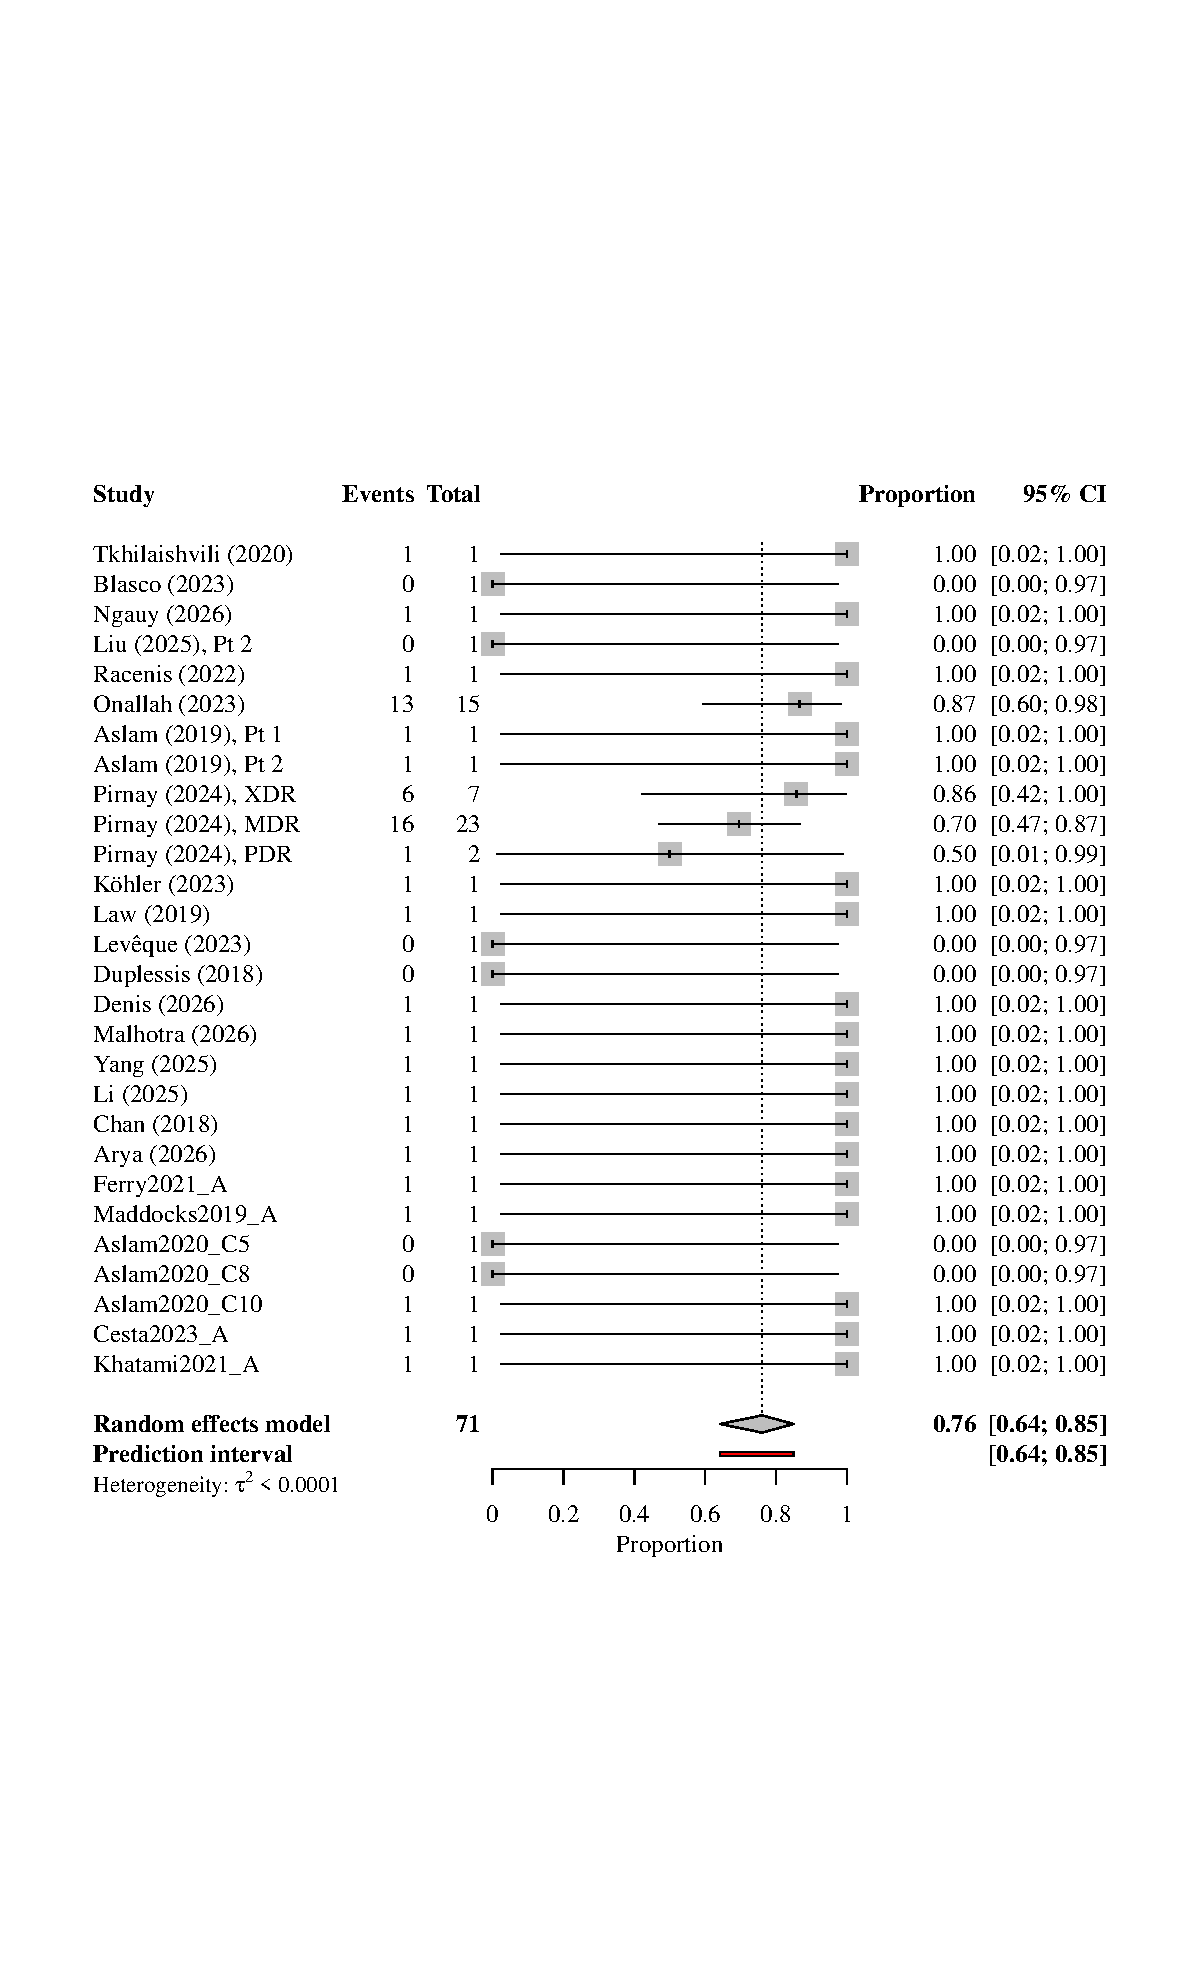
\includegraphics[width=0.8\textwidth]{figures/phage_therapy_mdr_pseudomonas/forest_clinical_success_overall.pdf}
\caption{Forest plot: pooled clinical success, overall (secondary/contextual). Each row is one of the 20 studies contributing clinical-success data (67 patients); markers show the study-specific proportion with 95\% CI, the diamond shows the GLMM pooled estimate (77.6\%, 95\% CI 65.4--86.4\%). Reported for comparability with prior non-stratified syntheses, not as this review's primary estimand. Source: \texttt{scripts/R/07\_figures.R}.}
\label{fig:forest-success-overall}
\end{figure}

\begin{figure}[htbp]
\centering
\begin{subfigure}{0.48\textwidth}
\centering
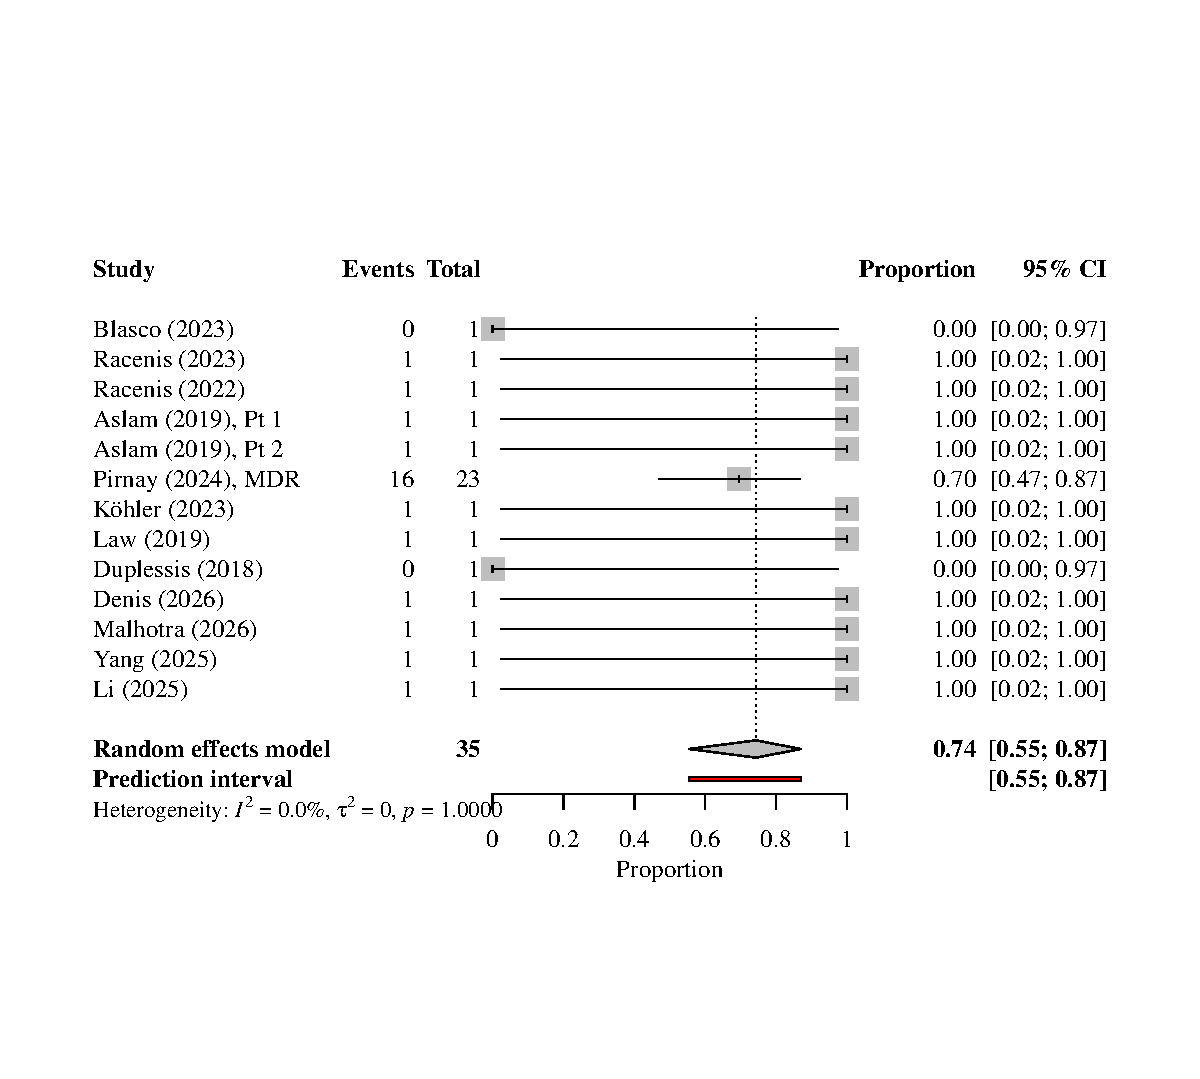
\includegraphics[width=\textwidth]{figures/phage_therapy_mdr_pseudomonas/forest_clinical_success_resistance_MDR.pdf}
\caption{MDR resistance stratum}
\label{fig:forest-success-mdr-a}
\end{subfigure}
\hfill
\begin{subfigure}{0.48\textwidth}
\centering
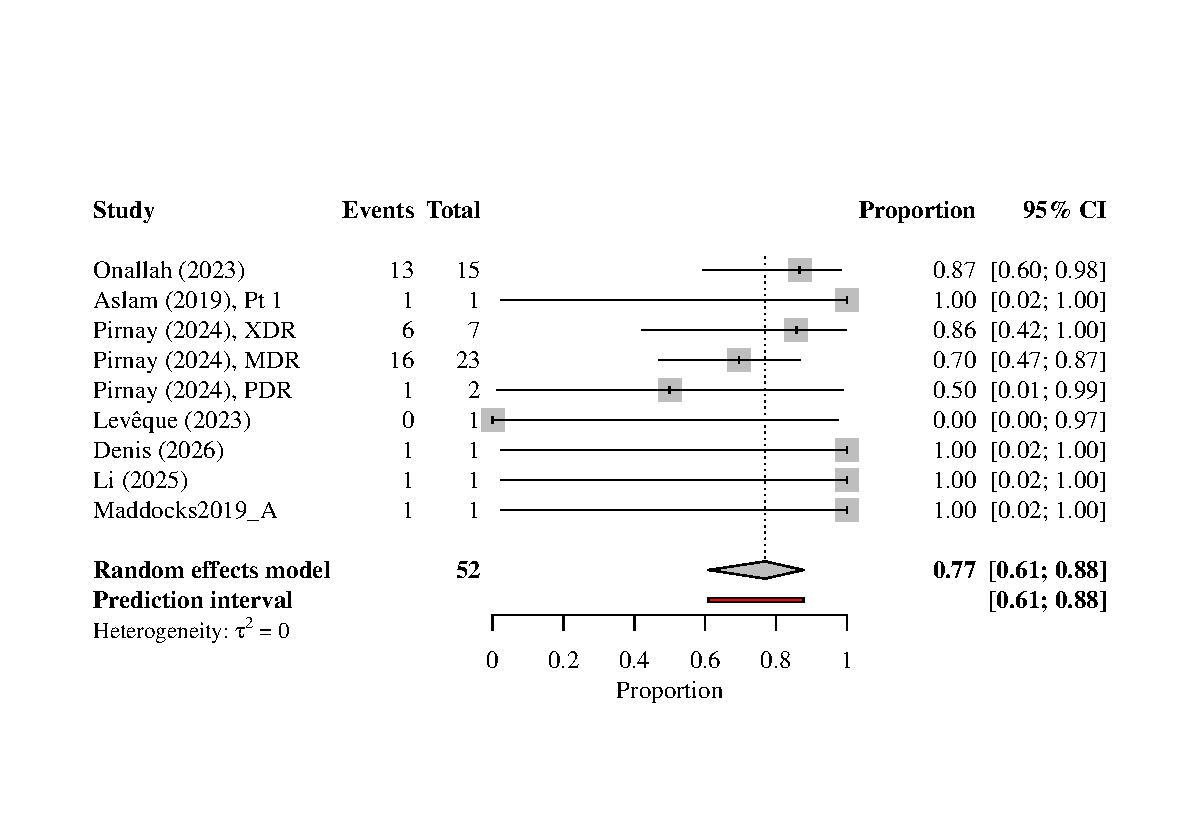
\includegraphics[width=\textwidth]{figures/phage_therapy_mdr_pseudomonas/forest_clinical_success_route_other.pdf}
\caption{Route: ``other'' (multi-route)}
\label{fig:forest-success-mdr-b}
\end{subfigure}
\caption{Forest plots: two stratified cells meeting the pooling threshold. Panel (a): clinical success among the 14 studies (37 patients) classified MDR (75.7\%, 95\% CI 57.8--87.6\%) --- a single-cohort-dominated estimate that clears the pooling threshold only under author-reported resistance labels (Section~\ref{sec:results-robustness}). Panel (b): clinical success among the 7--8 studies (38--53 patients depending on outcome) coded a multi-route or otherwise unclassifiable ("other") route (77.4\%, 95\% CI 61.9--87.8\% for clinical success). XDR, PDR, and every specific single route fell below threshold and are not plotted; see \Cref{tab:not-pooled}. Source: \texttt{scripts/R/07\_figures.R}.}
\label{fig:forest-success-mdr}
\end{figure}

Pooled safety (at least one adverse event), across 20 studies (81 patients), is 19.1\% (95\% CI 9.6--34.4\%; $\tau^2=0.085$; \Cref{fig:forest-safety-overall}). Leave-one-out does not flag the \emph{overall} safety estimate as sensitive to any single study's removal, though the MDR-specific safety estimate, the mortality-specific estimate in both the MDR and not-classifiable resistance strata, and the route-``other'' safety estimate remain sensitive to removing \citeauthor{Pirnay2024_natmicrobiol} (MDR, route-``other'') or \citeauthor{Jault2019_phagoburn} (not-classifiable mortality) specifically, collapsing to a value indistinguishable from zero on removal. The sensitivity models bracket the GLMM: Freeman-Tukey gives 7.9\% and logit-DerSimonian-Laird gives 26.8\% against the GLMM's 19.1\% (\Cref{tab:sensitivity}), and the fixed-effect model converges at 26.8\% too. Even so, the MDR- and route-specific safety/mortality estimates, and the two not-classifiable safety/mortality cells, should be read as resting heavily on one or two dominant sources, not as an even-weighted synthesis across independent studies (Section~\ref{sec:results-robustness}).

\begin{figure}[htbp]
\centering
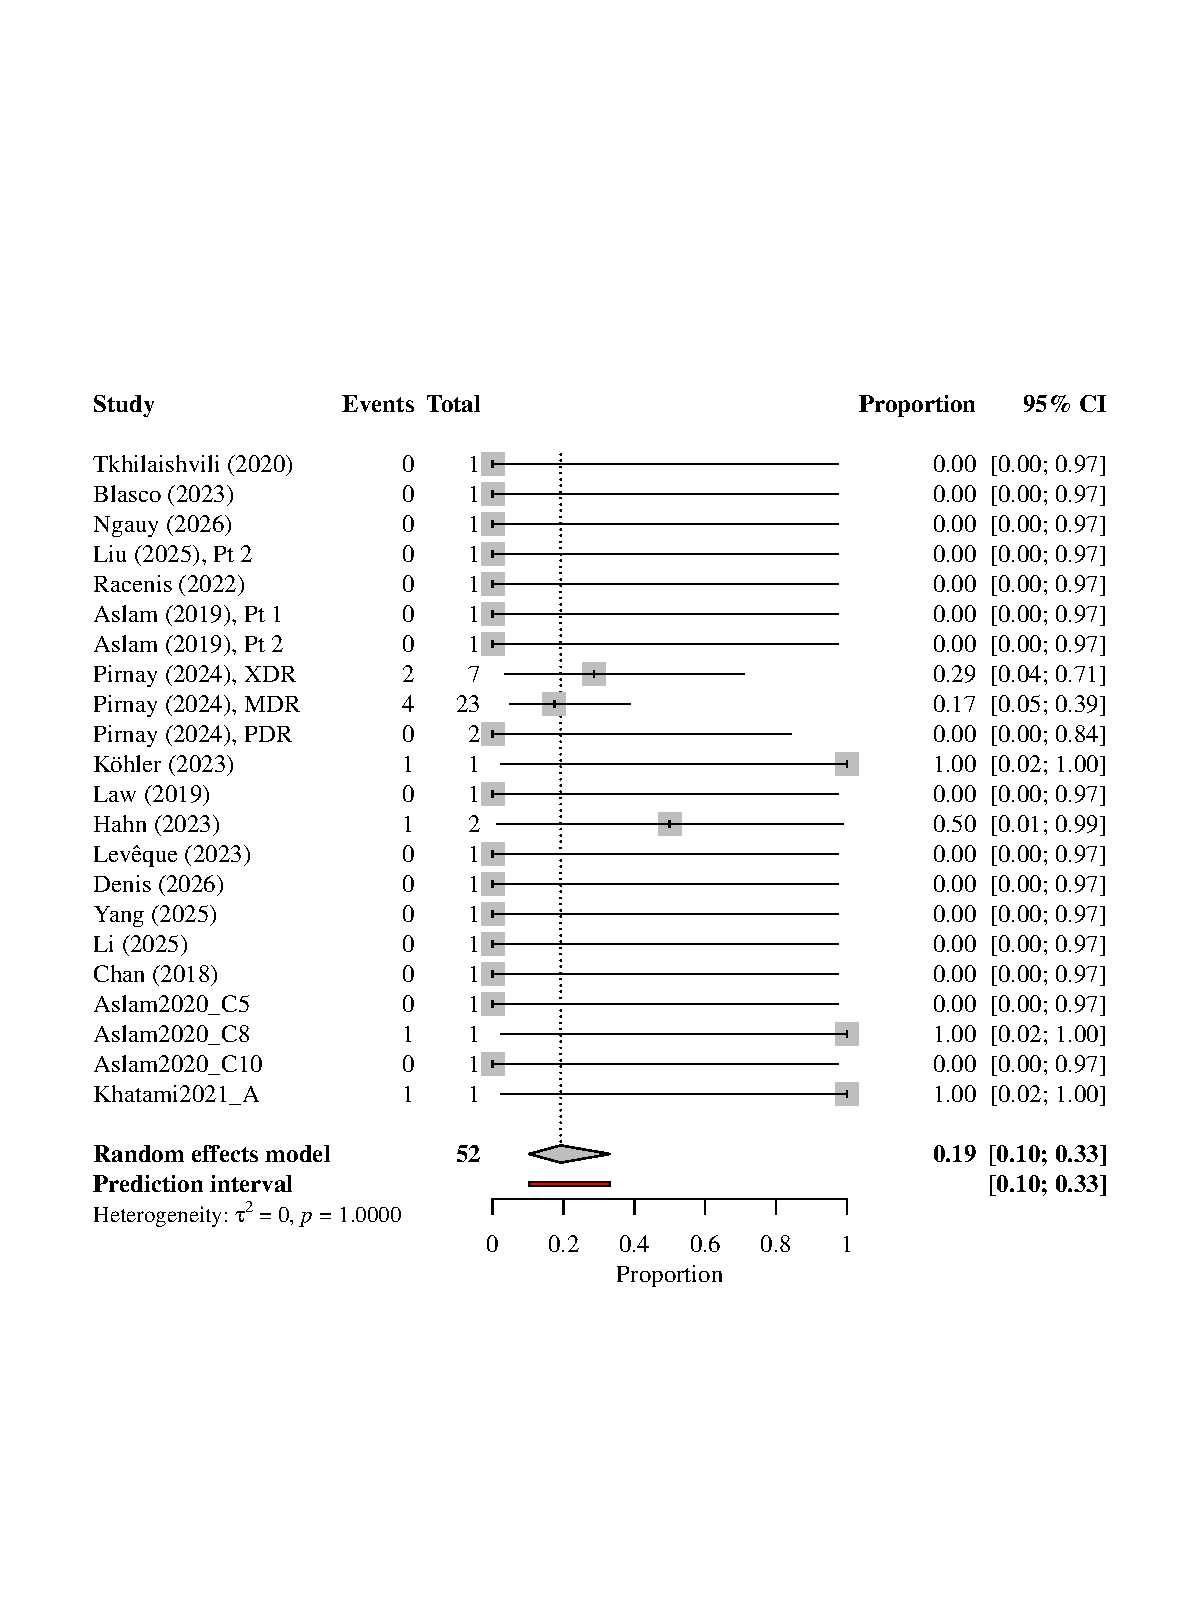
\includegraphics[width=0.8\textwidth]{figures/phage_therapy_mdr_pseudomonas/forest_safety_overall.pdf}
\caption{Forest plot: pooled safety (at least one adverse event), overall (secondary/contextual). Each row is one of the 20 studies contributing safety data (81 patients); the GLMM diamond shows 19.1\% (95\% CI 9.6--34.4\%). Leave-one-out (Section~\ref{sec:results-robustness}) no longer flags this specific estimate as sensitive to any single study's removal, though the MDR- and route-specific safety estimates remain so. Source: \texttt{scripts/R/07\_figures.R}.}
\label{fig:forest-safety-overall}
\end{figure}

\subsection{Sensitivity and Robustness Analyses}
\label{sec:results-robustness}

Transformation and model choice changes the pooled estimate by more than 5 percentage points in 12 of the 15 pooled cells; the three cells below the flag threshold are eradication overall, not-classifiable mortality, and the inhaled/nebulized safety cell (\Cref{tab:sensitivity}). Leave-one-out removal of each (arm, cell) combination shifts a pooled estimate outside its full-sample CI in exactly 4 cases: removing \citeauthor{Pirnay2024_natmicrobiol} (\citeyear{Pirnay2024_natmicrobiol}) collapses the MDR-specific safety and mortality estimates and the route-"other" safety estimate to a value numerically indistinguishable from zero, and removing \citeauthor{Jault2019_phagoburn} (\citeyear{Jault2019_phagoburn}) does the same to the not-classifiable resistance stratum's new mortality estimate. Notably, the \emph{overall} safety and mortality estimates are not shifted outside their CIs by any single-study removal. The same removals do \emph{not} overturn the clinical-success or eradication estimates in any stratum, including MDR, where Pirnay supplies the large majority of pooled patients (Section~\ref{sec:results-synthesis}) --- the instability is confined to the safety/mortality outcomes in specific strata rather than a general fragility of the MDR or not-classifiable pools. The Hartung-Knapp-Sidik-Jonkman adjustment \parencite{IntHout2014_hksj} widens the CI relative to a Wald interval in every pooled cell, confirming it as the more conservative, appropriate choice given the small number of studies per cell. Robust-variance clustering by study changes standard errors in different directions depending on the cell: eradication in the route-"other" stratum narrows substantially (naive SE 0.342 to RVE SE 0.098), while mortality in the same stratum widens (0.457 to 0.514), so the naive-independence assumption is neither confirmed nor cleanly refuted as a uniform source of bias. A classification-sensitivity check restricting to independently-verified resistance labels only (rather than the primary analysis's mix of independently-verified and author-reported labels) is materially informative for the new MDR finding: under independently-verified-only classification, the MDR cell drops to $k=3$ studies and $N=4$ patients and no longer meets the pooling threshold for any outcome --- the MDR pooled estimate reported above depends substantially on author-reported (not independently re-derived) classifications, most of them from \citeauthor{Pirnay2024_natmicrobiol}'s own per-patient antibiogram-based labels, which this review team did not re-verify against raw susceptibility data.

\begin{table}[htbp]
\centering
\scriptsize
\setlength{\tabcolsep}{3pt}
\begin{threeparttable}
\caption{Sensitivity of pooled estimates to transformation and pooling-model choice}
\label{tab:sensitivity}
\begin{tabular}{llc}
\toprule
Stratum & Model & Pooled proportion [95\% CI] \\
\midrule
Clinical success -- Overall & GLMM (primary or NA if non-convergent) & 77.6\% [65.4\%, 86.4\%] \\
Clinical success -- Overall & Freeman-Tukey double-arcsine DL & 88.4\% [76.0\%, 97.4\%] \\
Clinical success -- Overall & Logit DerSimonian-Laird & 70.9\% [63.7\%, 77.2\%] \\
Clinical success -- Overall & Fixed-effect (logit) & 70.9\% [59.6\%, 80.0\%] \\
Safety (>=1 AE) -- Overall & GLMM (primary or NA if non-convergent) & 16.0\% [7.8\%, 29.9\%] \\
Safety (>=1 AE) -- Overall & Freeman-Tukey double-arcsine DL & 5.2\% [0.5\%, 13.0\%] \\
Safety (>=1 AE) -- Overall & Logit DerSimonian-Laird & 24.8\% [20.4\%, 29.9\%] \\
Safety (>=1 AE) -- Overall & Fixed-effect (logit) & 24.8\% [15.7\%, 37.0\%] \\
Eradication -- Overall & GLMM (primary or NA if non-convergent) & 52.9\% [27.8\%, 76.6\%] \\
Eradication -- Overall & Freeman-Tukey double-arcsine DL & 50.8\% [24.5\%, 76.9\%] \\
Eradication -- Overall & Logit DerSimonian-Laird & 55.7\% [45.0\%, 65.9\%] \\
Eradication -- Overall & Fixed-effect (logit) & 55.7\% [43.1\%, 67.6\%] \\
Mortality -- Overall & GLMM (primary or NA if non-convergent) & 12.7\% [6.3\%, 24.1\%] \\
Mortality -- Overall & Freeman-Tukey double-arcsine DL & 1.8\% [0.0\%, 11.0\%] \\
Mortality -- Overall & Logit DerSimonian-Laird & 24.8\% [18.1\%, 33.0\%] \\
Mortality -- Overall & Fixed-effect (logit) & 24.8\% [15.9\%, 36.5\%] \\
Clinical success -- Resistance: MDR & GLMM (primary or NA if non-convergent) & 75.7\% [57.8\%, 87.6\%] \\
Clinical success -- Resistance: MDR & Freeman-Tukey double-arcsine DL & 86.7\% [70.4\%, 98.0\%] \\
Clinical success -- Resistance: MDR & Logit DerSimonian-Laird & 69.1\% [61.9\%, 75.4\%] \\
Clinical success -- Resistance: MDR & Fixed-effect (logit) & 69.1\% [54.7\%, 80.6\%] \\
Safety (>=1 AE) -- Resistance: MDR & GLMM (primary or NA if non-convergent) & 16.7\% [7.0\%, 34.6\%] \\
Safety (>=1 AE) -- Resistance: MDR & Freeman-Tukey double-arcsine DL & 5.1\% [0.0\%, 16.9\%] \\
Safety (>=1 AE) -- Resistance: MDR & Logit DerSimonian-Laird & 24.7\% [18.1\%, 32.7\%] \\
Safety (>=1 AE) -- Resistance: MDR & Fixed-effect (logit) & 24.7\% [14.0\%, 39.6\%] \\
Eradication -- Resistance: MDR & GLMM (primary or NA if non-convergent) & 58.1\% [12.5\%, 93.1\%] \\
Eradication -- Resistance: MDR & Freeman-Tukey double-arcsine DL & 50.7\% [15.3\%, 85.8\%] \\
Eradication -- Resistance: MDR & Logit DerSimonian-Laird & 55.5\% [41.9\%, 68.3\%] \\
Eradication -- Resistance: MDR & Fixed-effect (logit) & 55.5\% [40.7\%, 69.3\%] \\
Mortality -- Resistance: MDR & GLMM (primary or NA if non-convergent) & 6.5\% [1.9\%, 19.8\%] \\
Mortality -- Resistance: MDR & Freeman-Tukey double-arcsine DL & 0.0\% [0.0\%, 2.2\%] \\
Mortality -- Resistance: MDR & Logit DerSimonian-Laird & 19.7\% [13.8\%, 27.4\%] \\
Mortality -- Resistance: MDR & Fixed-effect (logit) & 19.7\% [10.9\%, 33.0\%] \\
Clinical success -- Route: other & GLMM (primary or NA if non-convergent) & 77.4\% [61.9\%, 87.8\%] \\
Clinical success -- Route: other & Freeman-Tukey double-arcsine DL & 87.4\% [72.6\%, 97.9\%] \\
Clinical success -- Route: other & Logit DerSimonian-Laird & 73.6\% [63.2\%, 81.8\%] \\
Clinical success -- Route: other & Fixed-effect (logit) & 73.6\% [60.1\%, 83.7\%] \\
Safety (>=1 AE) -- Route: other & GLMM (primary or NA if non-convergent) & 15.8\% [6.3\%, 34.3\%] \\
Safety (>=1 AE) -- Route: other & Freeman-Tukey double-arcsine DL & 4.8\% [0.8\%, 10.8\%] \\
Safety (>=1 AE) -- Route: other & Logit DerSimonian-Laird & 21.5\% [17.9\%, 25.5\%] \\
Safety (>=1 AE) -- Route: other & Fixed-effect (logit) & 21.5\% [11.7\%, 36.0\%] \\
Eradication -- Route: other & GLMM (primary or NA if non-convergent) & 63.2\% [44.1\%, 78.8\%] \\
Eradication -- Route: other & Freeman-Tukey double-arcsine DL & 68.6\% [46.3\%, 88.1\%] \\
Eradication -- Route: other & Logit DerSimonian-Laird & 61.6\% [50.7\%, 71.4\%] \\
Eradication -- Route: other & Fixed-effect (logit) & 61.6\% [46.0\%, 75.1\%] \\
Mortality -- Route: other & GLMM (primary or NA if non-convergent) & 16.0\% [3.6\%, 48.9\%] \\
Mortality -- Route: other & Freeman-Tukey double-arcsine DL & 5.9\% [0.0\%, 31.2\%] \\
Mortality -- Route: other & Logit DerSimonian-Laird & 23.2\% [11.3\%, 41.6\%] \\
Mortality -- Route: other & Fixed-effect (logit) & 23.2\% [11.9\%, 40.3\%] \\
\bottomrule
\end{tabular}

\begin{tablenotes}
\small
\item \textit{Notes:} All 15 cells meeting the pre-specified pooling threshold (\Cref{tab:pooled-estimates}), compared across the primary random-effects binomial-normal GLMM (logit link), the Freeman-Tukey double-arcsine transformation with DerSimonian-Laird pooling \parencite{FreemanTukey1950,DerSimonianLaird1986}, a logit transformation with DerSimonian-Laird pooling, and a fixed-effect (logit) model. Divergence exceeding 5 percentage points between GLMM and the sensitivity models is reported as a finding in the text (Section~\ref{sec:results-robustness}), not a footnote. Source: \texttt{scripts/R/05\_robustness.R}, \texttt{08\_tables.R}.
\end{tablenotes}
\end{threeparttable}
\end{table}

An appendix-only relaxation of the threshold to at least 2 studies and 10 patients (\Cref{tab:threshold-relaxation}) newly qualifies several cells beyond the primary set --- clinical success in the not-classifiable resistance stratum ($k=2$, $N=16$), safety and mortality in the topical/local route ($k=5$, $N=18$ each, the topical/local arms enlarged by the newly added \citeauthor{Chan2018_omko1_emph} case), and all four XDR outcome cells ($k=4$, $N=10$ each, having just reached the ten-patient relaxed floor as the corpus grew) --- while PDR and intravenous remain below even the relaxed threshold. (Safety in the inhaled/nebulized route, previously below threshold, now clears the \emph{primary} threshold and appears in \Cref{tab:pooled-estimates} rather than here.) These estimates are reported only to show that the primary threshold is itself consequential; none is promoted to a primary result. A study-design-stratified comparison (RCT/cohort vs.\ case report/series) found no significant subgroup difference for clinical success (Q-between $p=0.285$), and a collapsed systemic-versus-local (2-category) route taxonomy likewise found none ($p=0.53$). A geographic-concentration exclusion of the Belgium and Israel cohorts --- which together supply the two largest sources in the corpus, \citeauthor{Pirnay2024_natmicrobiol} and \citeauthor{Onallah2023_med} --- now leaves all four overall outcomes above the pooling threshold: clinical success (0.776, essentially unchanged at 0.800 once excluded), safety (0.191 falling to 0.140), eradication (0.551 rising to 0.685), and mortality (0.105 falling to 0.037). That the enlarged corpus retains all four overall estimates even without its two dominant cohorts is a robustness improvement over earlier versions of this review, in which removing them pushed clinical success (and, earlier still, eradication) below the pooling threshold. A Liu et al.\ reuse-tier transparency check confirms every one of the 30 pooling-eligible rows is coded \texttt{data\_provenance == independently-extracted} (Section~\ref{sec:methods-extraction}); no row uses Tier-3 (directly adopted) data, so the independently-extracted-only and all-rows pooled estimates are identical by construction, reported as a transparency confirmation rather than a contrast.

\begin{table}[htbp]
\centering
\scriptsize
\setlength{\tabcolsep}{3pt}
\begin{threeparttable}
\caption{Appendix: effect of relaxing the pooling threshold to $k \geq 2$ studies and $N \geq 10$ patients}
\label{tab:threshold-relaxation}
\begin{tabular}{lllccl}
\toprule
Outcome -- Stratum & Primary$^a$ & Relaxed$^b$ & $k$ (relaxed) & $N$ (relaxed) & Flag \\
\midrule
Clinical success -- Overall & POOLED & POOLED & 23 & 71 &  \\
Safety (>=1 AE) -- Overall & POOLED & POOLED & 18 & 53 &  \\
Eradication -- Overall & POOLED & POOLED & 20 & 60 &  \\
Mortality -- Overall & POOLED & POOLED & 24 & 67 &  \\
Clinical success -- Resistance: MDR & POOLED & POOLED & 15 & 38 &  \\
Clinical success -- Resistance: NC & NOT\_POOLED & POOLED & 4 & 19 & NEW (relaxed) \\
Clinical success -- Resistance: PDR & NOT\_POOLED & NOT\_POOLED & 3 & 4 &  \\
Clinical success -- Resistance: XDR & NOT\_POOLED & POOLED & 4 & 10 & NEW (relaxed) \\
Safety (>=1 AE) -- Resistance: MDR & POOLED & POOLED & 13 & 37 &  \\
Safety (>=1 AE) -- Resistance: NC & NOT\_POOLED & NOT\_POOLED & 1 & 2 &  \\
Safety (>=1 AE) -- Resistance: PDR & NOT\_POOLED & NOT\_POOLED & 3 & 4 &  \\
Safety (>=1 AE) -- Resistance: XDR & NOT\_POOLED & POOLED & 4 & 10 & NEW (relaxed) \\
Eradication -- Resistance: MDR & POOLED & POOLED & 14 & 43 &  \\
Eradication -- Resistance: NC & NOT\_POOLED & NOT\_POOLED & 1 & 1 &  \\
Eradication -- Resistance: PDR & NOT\_POOLED & NOT\_POOLED & 4 & 6 &  \\
Eradication -- Resistance: XDR & NOT\_POOLED & POOLED & 4 & 10 & NEW (relaxed) \\
Mortality -- Resistance: MDR & POOLED & POOLED & 17 & 47 &  \\
Mortality -- Resistance: NC & NOT\_POOLED & NOT\_POOLED & 3 & 4 &  \\
Mortality -- Resistance: PDR & NOT\_POOLED & NOT\_POOLED & 4 & 6 &  \\
Mortality -- Resistance: XDR & NOT\_POOLED & POOLED & 4 & 10 & NEW (relaxed) \\
Clinical success -- Route: inhaled/nebulized & NOT\_POOLED & NOT\_POOLED & 2 & 2 &  \\
Clinical success -- Route: IV & NOT\_POOLED & NOT\_POOLED & 6 & 8 &  \\
Clinical success -- Route: other & POOLED & POOLED & 9 & 54 &  \\
Clinical success -- Route: topical/local & NOT\_POOLED & NOT\_POOLED & 5 & 5 &  \\
Safety (>=1 AE) -- Route: inhaled/nebulized & NOT\_POOLED & NOT\_POOLED & 3 & 4 &  \\
Safety (>=1 AE) -- Route: IV & NOT\_POOLED & NOT\_POOLED & 5 & 7 &  \\
Safety (>=1 AE) -- Route: other & POOLED & POOLED & 7 & 38 &  \\
Safety (>=1 AE) -- Route: topical/local & NOT\_POOLED & NOT\_POOLED & 4 & 4 &  \\
Eradication -- Route: inhaled/nebulized & NOT\_POOLED & NOT\_POOLED & 3 & 11 &  \\
Eradication -- Route: IV & NOT\_POOLED & NOT\_POOLED & 5 & 5 &  \\
Eradication -- Route: other & POOLED & POOLED & 8 & 39 &  \\
Eradication -- Route: topical/local & NOT\_POOLED & NOT\_POOLED & 4 & 4 &  \\
Mortality -- Route: inhaled/nebulized & NOT\_POOLED & NOT\_POOLED & 4 & 13 &  \\
Mortality -- Route: IV & NOT\_POOLED & NOT\_POOLED & 6 & 8 &  \\
Mortality -- Route: other & POOLED & POOLED & 8 & 39 &  \\
Mortality -- Route: topical/local & NOT\_POOLED & NOT\_POOLED & 5 & 5 &  \\
\bottomrule
\end{tabular}

\begin{tablenotes}
\small
\item \textit{Notes:} Supplementary sensitivity check, not a primary result. Compares each cell's pooling status under the primary threshold ($k \geq 3$, $N \geq 20$) against a relaxed threshold ($k \geq 2$, $N \geq 10$). Cells flagged "NEW (relaxed)" are reported for transparency about threshold sensitivity and are not promoted to \Cref{tab:pooled-estimates} or cited elsewhere as primary findings. Source: \texttt{scripts/R/05\_robustness.R}, \texttt{08\_tables.R}.
\item[a] Pooling status under the primary threshold ($k \geq 3$ studies, $N \geq 20$ patients).
\item[b] Pooling status under the relaxed threshold ($k \geq 2$ studies, $N \geq 10$ patients).
\end{tablenotes}
\end{threeparttable}
\end{table}

\subsection{Falsification and Negative-Control Checks}
\label{sec:results-falsification}

Most of the six pre-specified falsification checks are null or pass as expected. A meta-regression of transformed clinical success on publication year found no secular trend (logit-scale coefficient $0.030$, $p=0.81$), arguing against a reporting-drift explanation. A cross-tabulation of route by resistance class by geographic source found no route confined to a single region, arguing against a route effect that is actually a single-center signature. The one check that does not fully pass is the journal-tier comparison: high-tier journals report a higher pooled clinical-success proportion (79.6\%, 8 studies) than mid-tier journals (69.2\%, 12 studies), a roughly 10-percentage-point gap. With only two tiers and small per-tier counts this is not formally tested and should not be over-read, but the gradient is in the direction a selective-reporting or editorial-selection effect would produce, and is reported here as a mild caution rather than a clean pass. The length-of-hospitalization comparison remains not applicable: only 1 of the 30 arms reports a value, too sparse for even a qualitative check.

Peters' regression test for funnel-plot asymmetry, applied to the four outcome-overall cells with at least 10 studies as pre-specified, is non-significant for every tested outcome: clinical success ($p=0.66$), safety ($p=0.38$), eradication ($p=0.82$), and mortality ($p=0.24$; \Cref{fig:funnel-eyeball}). These four outcome-overall cells are the only ones that can support the test; the MDR-specific and other resistance-stratified cells have too few studies for Peters' regression and return no estimate (NA), so no small-study test is reported for them. Peters' test replaces the Egger's linear regression an earlier version of this review applied here, and the substitution reverses the earlier apparent finding. Egger's test is invalid for a meta-analysis of proportions: the standard error is a deterministic function of the proportion and manufactures funnel asymmetry near the 0/1 boundary. The earlier ``mortality signal'' ($p=0.02$ under Egger's) was an artifact of exactly that failure mode --- a mortality funnel dominated by single-patient arms at 0\% and two at 100\% --- not genuine small-study bias; under the appropriate Peters' test mortality asymmetry is not significant ($p=0.24$), and no outcome is. We read this as reassurance, but weak reassurance: non-significance in a corpus of 30 study-arms that remains small and, as Section~\ref{sec:results-robustness}'s leave-one-out and classification-sensitivity checks show, dependent on one or two dominant sources in several strata, is the absence of a detectable small-study effect under a test the data can properly support, not a clean acquittal.

\begin{figure}[htbp]
\centering
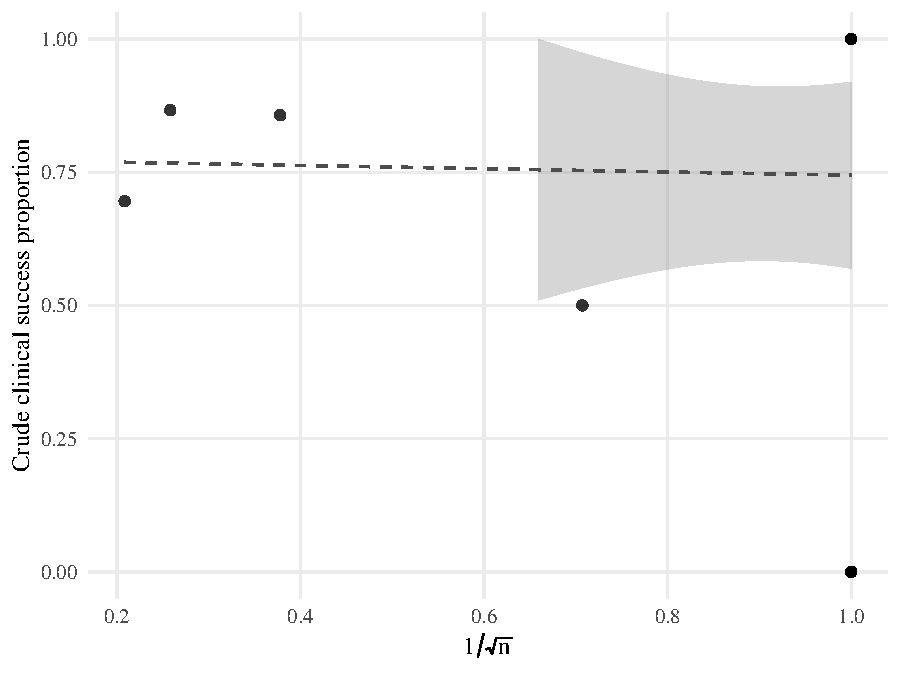
\includegraphics[width=0.8\textwidth]{figures/phage_therapy_mdr_pseudomonas/small_study_eyeball.pdf}
\caption{Small-study effects: crude proportion versus $1/\sqrt{n}$. Each point is one pooling-eligible study-arm; the $x$-axis is the inverse square root of arm sample size (a proxy for precision), the $y$-axis is the arm's crude, untransformed outcome proportion. A visual complement to the formal Peters' regression test (clinical success $p=0.66$, safety $p=0.38$, eradication $p=0.82$, mortality $p=0.24$; none significant), applied to the four outcome-overall cells with at least 10 studies per the pre-specified threshold; the resistance-stratified cells have too few studies to support the test. Source: \texttt{scripts/R/06\_falsification.R}, \texttt{07\_figures.R}.}
\label{fig:funnel-eyeball}
\end{figure}

\subsection{Certainty of Evidence (GRADE)}
\label{sec:results-grade}

Certainty of evidence was rated for all 15 pooled cells (Section~\ref{sec:methods-rob}). \textbf{Every cell is rated Very low.} That uniform verdict is not a formality: it follows from each cell starting at Low certainty --- the GRADE default for uncontrolled observational evidence, which is what a single-arm proportion drawn from compassionate-use case reports is --- and then being rated down at least twice more, so that all cells reach GRADE's floor. The practical implication is direct: none of the proportions reported above should be used to inform a treatment decision, and the review's contribution lies in mapping where evidence is absent rather than in the point estimates themselves.

The domain profile in \Cref{tab:grade} nonetheless discriminates sharply among cells, and that profile is more informative than the floored rating. Three cells carry the minimum burden of three downgrades --- overall safety, overall mortality, and the route-``other'' safety estimate --- each rated down once for risk of bias, once for the salvage-population indirectness common to every cell, and once for suspected publication bias, but not for inconsistency or imprecision. At the other extreme, MDR eradication accumulates seven downgrades' worth of problems (risk of bias, very serious inconsistency with a prediction interval spanning almost the entire 0--100\% range, indirectness, very serious imprecision, and publication bias), as do the not-classifiable safety cell and the inhaled/nebulized safety cell. The four clinical-success cells each take a second indirectness downgrade because success is defined by each primary study on its own terms across non-comparable infection syndromes (Section~\ref{sec:methods-eligibility}), so the pooled construct is not a single clinical outcome. Two structural downgrades apply to every cell without exception --- the compassionate-use salvage population, and publication bias --- and neither can be remedied by adding more case reports of the same kind.

\begin{table}[htbp]
\centering
\scriptsize
\setlength{\tabcolsep}{3pt}
\begin{threeparttable}
\caption{GRADE certainty of evidence for the 15 pooled outcome-stratum cells}
\label{tab:grade}
\begin{tabular}{lccclccccc l}
\toprule
Outcome -- Stratum & $k$ & Arms & $N$ & Pooled proportion [95\% CI] & RoB & Incons. & Indir. & Imprec. & Pub.\ bias & Certainty \\
\midrule
Clinical success -- Overall & 23 & 28 & 71 & 76.1\% [64.2, 84.9] & $-$1 & -- & $-$2 & -- & $-$1 & Very low \\
Safety (>=1 AE) -- Overall & 18 & 23 & 53 & 17.0\% [8.7, 30.4] & $-$1 & -- & $-$1 & -- & $-$1 & Very low \\
Eradication -- Overall & 20 & 24 & 60 & 55.1\% [29.4, 78.4] & $-$1 & $-$2 & $-$1 & $-$1 & $-$1 & Very low \\
Mortality -- Overall & 24 & 30 & 67 & 11.9\% [5.9, 22.7] & $-$1 & -- & $-$1 & -- & $-$1 & Very low \\
Clinical success -- Resistance: MDR & 15 & 16 & 38 & 73.7\% [56.1, 86.0] & $-$1 & -- & $-$2 & -- & $-$1 & Very low \\
Safety (>=1 AE) -- Resistance: MDR & 13 & 14 & 37 & 16.2\% [6.9, 33.7] & $-$1 & -- & $-$1 & -- & $-$1 & Very low \\
Eradication -- Resistance: MDR & 14 & 15 & 43 & 58.1\% [12.5, 93.1] & $-$1 & $-$2 & $-$1 & $-$2 & $-$1 & Very low \\
Mortality -- Resistance: MDR & 17 & 18 & 47 & 6.4\% [1.9, 19.4] & $-$1 & -- & $-$1 & -- & $-$1 & Very low \\
Clinical success -- Route: other & 9 & 11 & 54 & 77.8\% [62.8, 87.9] & $-$1 & -- & $-$2 & -- & $-$1 & Very low \\
Safety (>=1 AE) -- Route: other & 7 & 9 & 38 & 15.8\% [6.3, 34.3] & $-$1 & -- & $-$1 & -- & $-$1 & Very low \\
Eradication -- Route: other & 8 & 10 & 39 & 64.1\% [45.6, 79.2] & $-$1 & -- & $-$1 & $-$1 & $-$1 & Very low \\
Mortality -- Route: other & 8 & 10 & 39 & 15.4\% [6.2, 33.2] & $-$1 & -- & $-$1 & -- & $-$1 & Very low \\
\bottomrule
\end{tabular}

\begin{tablenotes}
\small
\item \textit{Notes:} All bodies of evidence start at \emph{Low} certainty (GRADE's default for observational evidence; every cell is an uncontrolled single-arm proportion) and are rated down across five domains. Domain columns give the number of certainty levels deducted; "--" denotes no downgrade. Certainty cannot fall below \emph{Very low} (GRADE's floor), so cells differing widely in their domain burden share the same final rating --- the profile, not the rating alone, carries the information. Rating rules are pre-specified and applied to each cell's own data rather than judged case by case: risk of bias from the share of patients contributed by single-patient case reports and the presence of the one High-risk-of-bias trial; inconsistency from the 95\% prediction-interval width; indirectness from the compassionate-use salvage population, with a second level for clinical success (defined per study across non-comparable syndromes); imprecision from the 95\% CI width; publication bias strongly suspected throughout (favourable-outcome reporting is intrinsic to a compassionate-use case-report literature and Peters' test cannot exclude it at this corpus size). No upgrade criterion applied. Source: \texttt{scripts/R/10\_grade.R}.
\end{tablenotes}
\end{threeparttable}
\end{table}


\section{Discussion}
\label{sec:discussion}

\subsection{Summary of Main Findings}
\label{sec:discussion-summary}

Pooled across the seventeen studies contributing clinical-success data, patients treated with bacteriophage therapy for MDR, XDR, or PDR \textit{P.\ aeruginosa} infections achieved clinical success in 76.9\% of cases (95\% CI 64.4--86.0\%; \Cref{fig:forest-success-overall}), directionally in line with earlier, non-stratified syntheses of this literature \parencite{ElHaddad2019_eskape,Uyttebroek2022_lancetid,Liu2025_ijaa}. That figure describes a compassionate-use population offered phage therapy after antibiotics had already failed, not a treatment effect measured against a comparator, and it is reported here as this review's secondary, contextual estimand rather than its headline finding (Section~\ref{sec:results-synthesis}). The headline finding is a partial success on the stratification this review was built to test: of the 37 outcome-stratum cells defined by resistance category, route, and modality, 16 met the pre-specified pooling threshold, including, for the first time, a clean resistance-specific stratum --- MDR, pooled across all four outcomes (11--14 studies, 35--44 patients depending on outcome) --- alongside a heterogeneous multi-route ``other'' bucket, safety and mortality within the residual not-classifiable resistance bucket, and, newly, safety and mortality in the inhaled/nebulized route (\Cref{tab:pooled-estimates,tab:not-pooled}). That MDR estimate answers part of the question this review set out to ask. It does not complete it: XDR (4 studies, 10 patients) and PDR (3--4 studies, 4--6 patients) remain below the patient threshold for every outcome, so the MDR-\emph{versus}-XDR comparison that motivated the stratification in the first place still cannot be made, and the entire monotherapy-versus-combination comparison still fell short entirely (0 antibiotic-monotherapy arms). This review's contribution is documenting exactly which parts of that stratification the evidence can and cannot yet support -- neither forcing an estimate it cannot bear nor dismissing the one clean success as noise.

\subsection{Comparison with Prior Syntheses}
\label{sec:discussion-comparison}

\textcite{ElHaddad2019_eskape}'s review of ESKAPE-pathogen phage therapy, \textcite{Uyttebroek2022_lancetid}'s larger \textit{Lancet Infectious Diseases} synthesis, and \textcite{Liu2025_ijaa}'s 130-study individual-patient-data meta-analysis each report favorable pooled outcomes for phage therapy broadly, consistent in direction with the success proportions found here, though none restricts its evidence base to \textit{P.\ aeruginosa} specifically or reports a directly comparable resistance- or pathogen-specific figure against which 76.9\% (overall) or 74.3\% (MDR-specific) could be checked numerically. What none of the three does is stratify by resistance category or route. This review can now do so partially: the MDR-specific pooled estimate (74.3\% clinical success, 95\% CI 55.4--87.0\%) is, to our knowledge, the first resistance-stratified pooled proportion for phage therapy in \textit{P.\ aeruginosa} specifically to clear a pre-specified evidentiary threshold. It remains an incomplete answer to the question that motivated the stratification --- a clinician still cannot compare it against an XDR- or PDR-specific figure, since neither clears the same threshold, and combination-versus-monotherapy remains entirely unanswerable (zero antibiotic-monotherapy arms) --- but identifying, cell by cell, which of those comparisons the published record can and cannot yet support is where this review adds something those three broader syntheses did not attempt.

\subsection{Safety Findings and Small-Study Effects}
\label{sec:discussion-safety}

The pooled safety estimate illustrates a problem with this literature more broadly, not only with this review's own numbers. The GLMM estimate (19.4\%, 95\% CI 10.0--34.4\%; Section~\ref{sec:results-synthesis}) is bracketed by its sensitivity models (Freeman-Tukey 8.2\%, logit-DerSimonian-Laird and fixed-effect both 26.9\%), and leave-one-out does not flag the \emph{overall} safety estimate as sensitive to any single study's removal. The MDR-specific safety and mortality estimates, the route-``other'' safety estimate, and the not-classifiable resistance stratum's mortality estimate remain sensitive, however, collapsing to a value indistinguishable from zero if \citeauthor{Pirnay2024_natmicrobiol} or \citeauthor{Jault2019_phagoburn} is removed. The MDR resistance stratum's pooled estimate therefore still leans on \citeauthor{Pirnay2024_natmicrobiol}'s cohort (23 of the 35 MDR patients in the clinical-success pool, 66\%; a smaller 56\% of the larger 41-patient MDR eradication pool), though the seven MDR arms added by the native Scopus search dilute that single-source dependence rather than deepen it, corroborated rather than counterbalanced by a set of much smaller studies.

Egger's test, applied to the outcome-overall cells with at least ten studies as pre-specified, now covers four outcomes. Three are non-significant --- clinical success ($p=0.26$), safety ($p=0.93$), and eradication ($p=0.37$; newly eligible now that eradication clears the ten-study minimum) --- but mortality is \textbf{significant} ($p=0.02$; \Cref{fig:funnel-eyeball}), and more so within the MDR stratum ($p=0.005$). The enlarged corpus thus reverses the earlier finding of no significant small-study asymmetry for at least one outcome: two small single-patient fatal case reports added by the native Scopus search (Lev\^eque et al.\ 2023; Duplessis et al.\ 2018) introduced exactly the asymmetry a mortality funnel is most prone to, with small studies reporting deaths clustering at the low-precision end. We read this as a signal that the pooled mortality figure (10.7\%) may if anything under-state true mortality, not as grounds to dismiss it --- it is one significant test among several non-significant ones in a still-small corpus. The other three outcomes' non-significant tests, meanwhile, remain weak reassurance rather than a clean acquittal: this corpus of 28 study-arms remains far smaller than any of the three prior syntheses discussed above, single-patient case reports still make up the largest design category (Section~\ref{sec:results-characteristics}), and the classification-sensitivity check (Section~\ref{sec:results-robustness}) shows the MDR finding depends on author-reported, not independently re-verified, resistance labels. Where a formal test does detect asymmetry, as for mortality, it should be taken seriously; where it does not, in a corpus this small and this dependent on one or two dominant sources, its silence is weak evidence of absence. We read the combined picture as narrowing rather than eliminating the small-study-effects concern a referee reviewing case-report-heavy evidence syntheses would be right to raise, and as reason to read the broader literature's high-success narrative, including the point estimates reported by \textcite{ElHaddad2019_eskape}, \textcite{Uyttebroek2022_lancetid}, and \textcite{Liu2025_ijaa}, with real caution.

\subsection{Limitations}
\label{sec:discussion-limitations}

Four limitations bear most directly on how much weight these estimates can carry. First, screening and extraction were conducted by a single reviewer, with a second reviewer's critique applied sequentially rather than concurrently (Sections~\ref{sec:methods-selection}--\ref{sec:methods-extraction}). That process caught several substantive errors before they entered, or after they had briefly entered, the analytic dataset --- a study initially catalogued as the closest candidate antibiotic-monotherapy comparator in this search, later confirmed on full text to contain zero \textit{P.\ aeruginosa} cases; a duplicate patient reported under two citations; and, most recently, two patients within \citeauthor{Pirnay2024_natmicrobiol}'s cohort whose resistance profile, once checked against per-patient data, turned out not to meet this review's own MDR/XDR/PDR eligibility criterion (Section~\ref{sec:results-characteristics}); and, from the native Scopus search, a single XDR case (Van Nieuwenhuyse et al., 2022) recognized as already counted within \citeauthor{Pirnay2024_natmicrobiol}'s Belgian-consortium cohort and excluded to prevent double-counting --- evidence the sequential-critique and re-extraction process catches real errors, and that the consortium double-counting risk is real and was actively screened for, but not a substitute for the dual-independent process a registered protocol would specify; a formal re-screen could still change which studies are included. Second, risk-of-bias ratings, now complete for all 29 study-arms (Section~\ref{sec:results-rob}), surface a genuine concern rather than resolve one. The trial that anchors this review's phage-monotherapy-adjacent evidence throughout --- PhagoBurn \parencite{Jault2019_phagoburn}, the only source with a phage-alone treatment arm compared against a non-phage standard-of-care --- rates \textbf{High risk of bias} on RoB2, driven by unmasked clinicians and by the trial stopping early for insufficient efficacy, both recognized bias-introducing deviations. This does not overturn anything already reported (PhagoBurn's clinical-success data were already excluded from pooling as a time-to-event, non-binary endpoint), but it does mean the one study in this corpus that most directly speaks to phage-versus-standard-of-care performance is also the one whose result should be trusted least on methodological grounds --- a genuinely unfavorable combination for a literature already short on comparative evidence. \citeauthor{Pirnay2024_natmicrobiol}'s cohort, by contrast, rates Low risk on the JBI checklist (explicitly consecutive, complete, transparent per-patient reporting), which if anything strengthens rather than weakens confidence in its now-dominant role in the MDR-specific estimates (Section~\ref{sec:discussion-safety}) --- the concern with that source is its weight in the pooled MDR estimate, not its individual quality. Third, the MDR resistance stratum --- this review's headline new finding --- still leans on a single source: \citeauthor{Pirnay2024_natmicrobiol} supplies 23 of the 35 MDR patients in the clinical-success pool (66\%; the several MDR arms added by the native Scopus search dilute this to 56\% in the larger 41-patient MDR eradication pool), and a classification-sensitivity check shows the stratum would fail the pooling threshold entirely (dropping to 3 studies, 4 patients) if restricted to independently-verified rather than author-reported resistance labels (Section~\ref{sec:results-robustness}). The MDR estimate should therefore be read as characterizing one large cohort's outcomes, corroborated in direction by a set of much smaller studies that now dilute --- but do not overturn --- its single-source dependence, not as an even-weighted synthesis across independent sources --- and XDR and PDR remain too sparse (10 and 4--6 patients respectively, depending on outcome) to pool at all, so the resistance-class comparison this review was built to answer is still only partially available. Fourth, the database coverage, though now materially improved, is not exhaustive. A native Scopus search (Section~\ref{sec:methods-search}) was added as a third core database alongside PubMed/MEDLINE and ClinicalTrials.gov and roughly doubled the pooling-eligible corpus (from 13 to 23 studies), adding ten studies the earlier PubMed-only rounds had missed and correcting one prior exclusion --- which both confirms the earlier coverage gap was real and material and largely closes it, since three searched databases meet a recognized minimum for a defensible PRISMA search and Scopus indexes much of EMBASE's content. EMBASE and Web of Science remain unsearched, but this is now a minor residual gap rather than a headline limitation. That the pooled eradication estimate has shifted by more than ten percentage points as studies were added across search rounds (standing at 55.5\% in the current corpus; \Cref{tab:pooled-estimates}) is nonetheless a direct reminder that the corpus is still small enough for a handful of additional records to move a headline figure, and completing a native EMBASE and Web of Science search would further stabilize the current estimates. Two data-handling limitations attach to the newly added studies: Chan et al.'s adverse-event data are reported only at the nine-patient cohort level and could not be attributed to the MDR-versus-PDR sub-groups, so they are recorded but not carried as a usable safety numerator (a documented data loss that, among other things, left the inhaled/nebulized route just short of the safety-pooling threshold); and Chan et al.'s compassionate cohort may share patients with the Yale CYPHY randomized trial, which is one reason CYPHY is kept out of pooling. Two further limitations are disclosed for completeness: no PROSPERO registration before extraction began (Section~\ref{sec:methods-protocol}), and a corpus, at 28 pooling-eligible arms and 106 patients, still too small to support most of the stratification it was designed to test --- the limitation this review treats as its central finding, not a footnote.

\subsection{Implications for Practice and Research}
\label{sec:discussion-implications}

For clinicians, the pooled proportions reported here should not inform a treatment decision: they summarize a referral-selected, salvage-therapy population, the resistance-class stratification that succeeded (MDR) rests overwhelmingly on a single cohort, and route- and modality-specific comparisons remain unanswerable. Most strata in this evidence base are expected to warrant a Very Low GRADE certainty rating once that assessment is completed (Section~\ref{sec:methods-rob}). For the field, this review's own experience points to three concrete needs: standardized outcome definitions across primary studies, since extracting ``clinical success'' required accepting each study's own definition because no consistent one exists (Section~\ref{sec:methods-eligibility}); comparative studies with a genuine antibiotic-monotherapy arm for \textit{P.\ aeruginosa} specifically, since despite a targeted search essentially none exist, and additional single-arm case reporting will not close that gap; and retrospective PROSPERO registration of this review disclosing the sequence in Section~\ref{sec:methods-protocol}, with prospective registration for any successor synthesis in this space.

\subsection{Conclusion}
\label{sec:discussion-conclusion}

What this review can defensibly claim is narrower than a single pooled percentage, but broader than a review that could not stratify by resistance category at all: bacteriophage therapy, used adjunctively in a small, referral-selected group of patients with MDR, XDR, or PDR \textit{P.\ aeruginosa} infections refractory to antibiotics, was associated with a high proportion of reported clinical success, including now a resistance-specific (MDR) estimate that, to our knowledge, is the first of its kind for this pathogen to clear a pre-specified evidentiary threshold --- though that estimate is itself dominated by one large cohort, not an even-weighted synthesis. What remains unknown is most, but no longer all, of what the stratification was designed to resolve: whether MDR, XDR, and PDR isolates respond differently is still unanswerable, since neither XDR nor PDR can yet be pooled at all, and whether route of administration or combination therapy matters remains equally open. The single most useful next step for this field is not another synthesis of the existing case-report literature, but two complementary efforts: independent replication of the MDR resistance-stratified estimate reported here in additional cohorts, so it no longer rests on one source, and a comparative study, ideally randomized, that pairs a genuine antibiotic-monotherapy arm with a phage-antibiotic combination arm in an MDR-, XDR-, or PDR-\textit{Pseudomonas}-specific population. Until both exist, the question this review set out to answer will remain only partially resolved.


\clearpage
\small
\printbibliography

\end{document}

% ====================================================================
% Preamble Deviations from .claude/rules/working-paper-format.md
% ====================================================================
% Dropped (econ-specific, not applicable to a systematic review):
%   - titlesec / titling / \pretitle-\posttitle custom title styling
%     (plain \maketitle is sufficient; no formal need for the econ
%     "thanks-footnote per author" convention with a single placeholder
%     author)
%   - amsthy + \newtheorem{theorem/proposition/corollary/lemma/
%     definition/hyp} and \argmax/\argmin/\norm/\1 macros: no formal
%     theory, propositions, or optimization notation appear anywhere
%     in this manuscript (theorist agent not dispatched for this
%     project per permissions.md CONDITIONAL flag)
%   - dsfont, mathtools, rotating, tabularx, pdflscape, tikz, float:
%     unused by any drafted section
%   - Custom L/C/R column types: no table in this paper uses them
%   - Custom citationcolor (0,127,255) + \DeclareCiteCommand color
%     overrides: replaced with hidelinks + colorlinks=false for a
%     plain black-text manuscript, closer to clinical-journal
%     convention than the azure citation-color aesthetic choice.
%     NOTE: xcolor itself is still loaded (added back after a
%     compile test) -- tabularray requires \color internals to be
%     defined even when no explicit color is applied in-document;
%     dropping xcolor entirely caused "Undefined control sequence
%     \set@color" errors during table rendering.
%   - JEL Codes: replaced with MeSH-style Keywords (Bacteriophages;
%     Pseudomonas aeruginosa; Drug Resistance, Multiple, Bacterial;
%     Phage Therapy; Systematic Reviews as Topic; Meta-Analysis as
%     Topic), per domain-profile.md and this task's instructions
% Kept (generically useful, field-agnostic):
%   - geometry, setspace/\doublespacing, fancyhdr, lmodern, microtype,
%     fontenc T1, amsmath/amssymb (needed for the GLMM display
%     equation in methods.tex), booktabs/threeparttable/tabularray
%     (+siunitx dependency), graphicx/subcaption/caption with
%     captionsetup, enumitem (methods.tex uses \begin{itemize} for
%     PICO eligibility criteria), biblatex+biber with natbib=true
%     (natbib compatibility kept even though only \parencite/
%     \textcite/\citeauthor/\citeyear are used in the drafted
%     sections, not \citet/\citep), hyperref loaded second-to-last,
%     cleveref loaded immediately after (results.tex and discussion.tex
%     use \Cref{} extensively for tables and figures)
% Title page: adapted to a single-author placeholder with an
%   institutional \thanks{} footnote (Universidad Catolica de Cuenca)
%   rather than the economics multi-author \quad-separated convention,
%   since no author list has been finalized.
% ====================================================================
